\documentclass{ifacconf}
\usepackage{standalone}
\usepackage{times}
\usepackage{float}
\usepackage{amsmath}
\usepackage{graphicx}      % include this line if your document contains figures
\usepackage{natbib}        % required for bibliography
%===========================================
%\documentclass[letterpaper, 11pt, onecolumn]{TemplateFiles/ieeeconf}
%\IEEEoverridecommandlockouts \overrideIEEEmargins 
%\pagestyle{plain}

%\usepackage[ruled,vlined,linesnumbered,boxruled]{algorithm2e}
%\usepackage{mathrsfs}
%\usepackage{graphicx}
%\usepackage{amsfonts}
%\usepackage{amsmath}
%\usepackage{amssymb}
%\usepackage{array}
%\usepackage{flafter}
%\usepackage{tabu}
%\usepackage{cite}
%\usepackage{subfigure}
%\usepackage{verbatim}
%\usepackage{bbm}
%\usepackage[usenames]{color}
%\usepackage[svgnames]{xcolor}

%\usepackage{balance}

%\usepackage{nicefrac}
%\usepackage{psfrag}
%\usepackage{umoline}
%\usepackage{hyperref}
%\usepackage{appendix} %[2009/09/02 v1.2b extra appendix facilities]
%\let\proof\relax
%\let\endproof\relax
%\usepackage{amsthm}	% This is needed for \newtheorem and proof environment.
% \usepackage{natbib} % for citing the papers with auther-year format in parantheses.
%\usepackage[numbers, sort]{natbib}

%\usepackage{etoolbox}

%\providecommand{\citet}[1]{\citeauthor{#1}\,[\citeyear{#1}]}
%\providecommand{\citep}[1]{\cite{#1}}

%\newtheorem{thm}{Theorem}
%\newtheorem{Def}{Definition}
%\newtheorem{Problem}{Problem}
%\newtheorem{Lem}{Lemma}
%\newtheorem{Cor}{Corollary}
%\newtheorem{assumption}{Assumption}
%\newtheorem{proposition}{Proposition}
%\newtheorem{definition}{Definition}
%\newtheorem{property}{Property}
%\newtheorem{Remark}{Remark}
%\newtheorem{exmp}{Example}[section]
%\newenvironment{proof}[1][Proof]{\begin{trivlist}
%\item[\hskip \labelsep {\bfseries #1}]}{\end{trivlist}}

%\newcommand{\TypeOfDoc}{IJRR} % This either can be TR or Conf or IJRR
%\newcommand{\FinalFlag}{No} % This either can be No or Accepted
%\newtoggle{finalpaper}
%\toggletrue{finalpaper}
%\togglefalse{finalpaper}

\graphicspath{{./figs/}}

%\allowdisplaybreaks[1]

%\newcommand{\kXX}[1]{\color{blue} XX #1 XX \color{black}}
%newcommand{\AXX}[1]{\color{purple} XX #1 XX \color{black}}
\newcommand{\aXX}[1]{\color{orange} #1  \color{black}}
\newcommand{\axx}[1]{\aXX{#1}}


\newcommand{\pr}[1]{\textbf{#1:} }

\newcommand{\codeline}[1]{\par{\ttfamily #1 \par}}  % This line is added because sth like this \newcommand{\initeali}{\verb|InitializeEdge|} does not work. For further details please check out this link % http://tex.stackexchange.com/questions/86071/newcommand-for-verbatim
% please do not delete above comments as it can be really confsing


%%%%%%%%%%%%%%%% symbols
\newcommand{\tv}{\varpi} % tube volume (edge tube volume)
\newcommand{\td}{\Gamma} % tube distance (edge tube distance)

%%%%%%%%%%%%%%%%%%%%%%%%%%%%%%%%%%%%%%%%%%%%%%%%%% To reduce pages
%\textfloatsep = 0pt
%\renewcommand{\baselinestretch}{0.96}
%%%%%%%%%%%%%%%%% Make bibs smaller
%\renewcommand{\IEEEbibitemsep}{0pt plus 2pt}
%\makeatletter
%\IEEEtriggercmd{\reset@font\normalfont\footnotesize}
%\makeatother
%\IEEEtriggeratref{1}

%%%%%%%%%%%%%%%%% margins
%\usepackage{geometry}
% \newcommand{\papermargin}{0.97in} % IEEE asks for 0.75 on all pages, but the first page
% %\newgeometry{top=0.75in,bottom=.75in,right=.75in,left=.75in}
% \newgeometry{top=\papermargin,bottom=\papermargin,right=\papermargin,left=\papermargin}
% \newgeometry{top=1.in,bottom=1.in,right=1.in,left=1.in}

\let\labelindent\relax
\usepackage{enumitem}

%% Additional packages
\usepackage{amsmath,amssymb,amsfonts}
\usepackage{mathtools}
\usepackage{subfigure}
\usepackage{graphicx}
\usepackage{color}
\usepackage{url}
%\usepackage[usenames,x11names]{xcolor}

\ifdefined\algorithm
% Don't load theorem style
\else
\usepackage[linesnumbered,vlined,ruled]{algorithm2e}
\fi

\usepackage{tikz,pgf} 
\usetikzlibrary{arrows,automata,shapes,calc,backgrounds,spy,positioning}
\usetikzlibrary{fit}

\usepackage{epstopdf}


 

%%% figure path
\graphicspath{{figures/}}
 
 
%% Roman, calligraphic, boldface, double barred letters
\newcommand{\RM}[1]{\mathrm{#1}}
\newcommand{\CA}[1]{\mathcal{#1}}
\newcommand{\BF}[1]{\mathbf{#1}}
\newcommand{\IT}[1]{\mathit{#1}}
\newcommand{\BB}[1]{\mathbb{#1}}
\newcommand{\TT}[1]{\mathtt{#1}}
\newcommand{\FK}[1]{\mathfrak{#1}}
\newcommand{\BS}[1]{\boldsymbol{#1}}


%% spaces 
\newcommand{\Real}{\BB{R}}
\newcommand{\Symb}{\mathcal S}
\newcommand{\borel}[1]{\mathcal{B}\left(#1\right)}


%%% Probability
\newcommand{\Ex}{\mathbf{E}}     % Probability of an event

\newcommand{\po}{\mathbf{P}}     % Probability of an event
\newcommand{\p}[1]{\po\left(#1\right)}     % Probability of an event
\renewcommand{\P}{\BF{P}}
\newcommand{\pd}[1]{p\left(#1\right)}     % Probability density  



%% Modelling symbols
%-------------MDP----------------------------
\newcommand{\MDP}{\mathsf{M}}
\newcommand{\POMDP}{\MDP_{\Z}}
\newcommand{\C}{\mathbf{C}}
\newcommand{\MB}{\mathsf{B}}

 
\newcommand{\X}{{\mathbb{X}}}  % State
\newcommand{\Z}{{\mathbb{Z}}}	% Observation space
\newcommand{\A}{{\mathbb{U}}} % Action space
\newcommand{\init}{\rho}
\newcommand{\tr}{t}


% product MDP
\renewcommand{\S}{{\mathbb{S}}}	% Observation space

\newcommand{\polb}{{\boldsymbol{\mu}}}
\renewcommand{\pol}{{\mu}}

\newcommand{\Y}{{\mathbb{Y}}}  % State

%-------------POMDP-----------------------------
\newcommand{\Hist}{{\mathsf{H}}}  %  History
\newcommand{\I}{{\mathsf{I}}}  %  History
\newcommand{\Belief}{b}
\newcommand{\trb}{\tr_\Belief}
\newcommand{\Xb}{{\X_\Belief}}  % State
\newcommand{\initb}{\init_\Belief}


% -----------------Refinement relation----------
\newcommand{\InF}{\mathcal{U}_{v}}
\newcommand{\Wt}{\mathbb{W}_{\tr}}

\newcommand{\grid}{\boldsymbol{\delta}}

%%% Logic 
%------------------Predicates-----------------------------------
\newcommand{\Fpred}{{\mathcal F}}
\newcommand{\Lab}{\mathsf{L}}
\newcommand{\Labset}{\mathcal{L}}

\newcommand{\alphabeth}{\Sigma}
\newcommand{\word}{{\boldsymbol{\pi}}} % words formed from the alphabeth
\newcommand{\letter}{\pi} % words formed from the alphabeth

\newcommand{\Bel}{{\mathbf {T}}}
\newcommand{\BelR}{{\mathbf {R}}}
\newcommand{\trunc}[2]{\operatorname{trunc}_{#1}\left(#2\right)}


%%% Temporal logic symbols
\newcommand{\notltl}{\neg}
\newcommand{\andltl}{\wedge}
\newcommand{\orltl}{\vee}
\newcommand{\Next}{\ensuremath{\bigcirc}}
\newcommand{\Always}{\ensuremath{\ \square\ }}
\newcommand{\Event}{\ensuremath{\ \diamondsuit\ }}
\newcommand{\Until}{\ \CA{U}\ }
\newcommand{\Implies}{\Rightarrow}
\newcommand{\Equiv}{\Leftrightarrow}
\newcommand{\True}{\top}
\newcommand{\False}{\perp}
\newcommand{\AP}{AP}
\newcommand{\pred}{\xi}


\newcommand{\eps}{\epsilon} \newcommand{\rel}{\mathcal{R}} % numbers option provides compact numerical references in the text. 

%----- Exotic words----- 
\newcommand{\buchi}{B\"uchi\ }

%% Symbols of automata
\newcommand{\PA}{\mathcal{P}} 
\newcommand{\BA}{\mathcal{B}}
\newcommand{\TS}{\mathcal{F}}
\newcommand{\Language}{\mathbf{Lang}} % Language?
\newcommand{\KA}{\mathcal{K}}
\newcommand{\RA}{\mathcal{R}}
\newcommand{\FSA}{\mathcal{A}}

\newcommand{\TSX}{\BB{V}_\TS}
\newcommand{\TSE}{\BB{E}_\TS}
\newcommand{\TSEE}{\BB{E}}

\newcommand{\DTL}{DTL~}

 % Custom operators
\newcommand{\norm}[1]{\left\| {#1} \right\|}
\newcommand{\norminf}[1]{\left\| {#1} \right\|_{\infty}}
\newcommand{\normeucl}[1]{\left\| {#1} \right\|_{2}}
\newcommand{\abs}[1]{\left| {#1} \right|} 
\DeclareMathOperator{\diag}{diag}



\ifdefined\theoremstyle
% Don't load theorem style:
%% There are a number of predefined theorem-like environments in
%% ifacconf.cls:
%%
%% \begin{thm} ... \end{thm}            % Theorem
%% \begin{lem} ... \end{lem}            % Lemma
%% \begin{claim} ... \end{claim}        % Claim
%% \begin{conj} ... \end{conj}          % Conjecture
%% \begin{cor} ... \end{cor}            % Corollary
%% \begin{fact} ... \end{fact}          % Fact
%% \begin{hypo} ... \end{hypo}          % Hypothesis
%% \begin{prop} ... \end{prop}          % Proposition
%% \begin{crit} ... \end{crit}          % Criterion
\newtheorem{theorem}[thm]{Theorem}
\newtheorem{lemma}[thm]{Lemma}
\newtheorem{definition}[thm]{Definition}


\newtheorem{example}{Example}

\else
\usepackage{amsthm}
\theoremstyle{plain}
\newtheorem{theorem}{Theorem}
\newtheorem{cor}{Corollary}
\newtheorem{prop}{Proposition}
\newtheorem{lemma}{Lemma}
\newtheorem{remark}{Remark}
\newtheorem{cond}{Condition}

\newtheorem{example}{Example}
\newtheorem{problem}{Problem}
\newtheorem{theorem}{Theorem}
\newtheorem{definition}[theorem]{Definition}
\fi

 
\pdfinfo{
   /Author (S.Haesaert et al.)
   /Title  (Formal abstraction of POMDPs for Distribution LTL)
   /CreationDate (D:20101201120000)
   /Subject (Formal abstraction)
   /Keywords (abstraction;POMDP)
}

% Table caption wrangling
\usepackage{etoolbox}
 

\usepackage[utf8]{inputenc}
\usepackage{pgfplots}
\usepackage{tikz}


\allowdisplaybreaks[1]
%% commenting
\newcommand{\red}[1]{{\color{red} #1}}
\renewcommand{\axx}[1]{{\color{orange} Ali: #1}}

\newcommand{\new}[1]{{\color{blue}#1}}
\newcommand{\ind}{\mathbf{1}}


\begin{document}


\begin{frontmatter}

\title{\huge Refinement-based temporal logic control of partially observable Markov decision processes }
%\thanks[footnoteinfo]{Sponsor and financial support acknowledgment
%goes here. Paper titles should be written in uppercase and lowercase
%letters, not all uppercase.}

\author[cal]{S. Haesaert} 
\author[cal]{P. Nilsson} 
\author[mit]{C.I. Vasile}
\author[jpl]{R. Thakker}
\author[jpl]{A. Agha}
\author[cal]{A.D.  Ames}
\author[cal]{R. M. Murray}



\address[cal]{California Institute of Technology, 
   Pasadena, CA 91125 USA} % (e-mail: \{haesaert,pettni,ames,murray\}@caltech ).}
\address[mit]{Massachusetts Institute of Technology, 
   Cambridge, MA 02139 USA}% (e-mail:  cvasile@mit.edu)}
\address[jpl]{Jet Propulsion Laboratory, 
   Pasadena, CA 91109 USA}% (e-mail: rohan.a.thakker@jpl.nasa.gov)} 
\maketitle
\begin{abstract}
The stochastic evolution of the partially observable Markov decision process (POMDP) can be modeled by transitions in an associated belief Markov decision process.
In this work, we consider the synthesis of controllers guaranteeing  specifications given in linear temporal logic on these belief models.
For this, we use an approximate  abstraction %of the belief space model
 suitable for the correct-by-construction control synthesis. By designing a control policy over the abstract model and refining it back to the original model, the computational issues involved with control synthesis on the original model can be circumvented. 
We leverage the notion of approximate stochastic simulation to quantify the deviation of the approximate models.  % The accuracy is expressed by the deviations in transition probability and by increasing non-determinism in the labeling of the Markov decision processes.
By compensating {\it a priori} for these deviations in the control synthesis for the abstract model, the guarantees are preserved for the refined control policy.
\end{abstract}
\begin{keyword} Belief space models,
correct-by-construction controller synthesis, Markov decision processes, partially observable
\end{keyword}

\end{frontmatter}
%%%%%%%%%%%%%%%%%%%%%%%%%%%%%%%%%%%%%%%%%%%%%%%%
%%%%%%%%%%%%%%%%%%%%%%%%%%%%%%%%%%%%%%%%%%%%%%%%
 
\section{Introduction }\label{subsec:intro}
\red{[Start with motivating the big picture (maybe with a picture)]}
The specification and design of controllers for navigation problems has  been shown to be well expressible via temporal logic specifications \citep{Murray2009}.      To represent the low-level control and decision making under motion and sensing uncertainty common in navigation problems, we model the system
    in its most generic and principled form as a Partially-Observable Markov Decision Process
    (POMDP)~\citep{Kaelbling98,Smallwood73}.
As in \citep{JonesDTL2013}, we specify the temporal logic properties with respect to their likelihood or uncertainty over the belief space of a POMDP.
In this work, we newly  leverage approximate stochastic simulation relations in the synthesis of  the control policy,  
 
 
 %Unlike the available work \citep{Vasile2016,JonesDTL2013}, we will synthesize control policies formally with guarantees. \axx{the last sentence need to be updated. let's talk about it in the meeting.}

%We define the belief space models of these POMDPs  to design controllers is commonly used for navigation problems.   

Given a specification $\psi$  written in linear temporal logic with propositions over the belief state of a POMDP, we are interested 
in the design of a policy $\pol$ such that  $\psi$ is satisfied with probability at least $p$.
%\[\po^\pol_\init(\MB\vDash \psi)\geq p.\]
%
In this paper, we approach the synthesis problem as follows. 
Firstly,  for a given belief MDP $\MB$ a finite state abstraction  $\tilde \MB$ is computed.
Secondly,  we compute a labeling-based approximate stochastic  simulation relation between the abstract belief space model  $\tilde{\MB}$ and the concrete model $\MB$.
 Then,  a $\delta$-robust policy for the abstract $\tilde{\MB}$ is computed  together with a stationary value function for the associated stochastic optimal control problem.
  Finally, the policy for the concrete belief space model is computed  as its refinement.





\subsubsection{Literature.}For probabilistic temporal logic properties  over finite state Markov decision processes %expressed in PCTL and CSL 
there exist several tools for policy synthesis and verification such as PRISM \citep{KNP11} and  Storm \citep{dehnert2017storm}. 
For Markov decision processes over uncountable state spaces,  the characterization of properties cannot in general be
attained analytically \citep{Abate1}, so an alternative is to approximate these models by simpler
processes that are prone to be mathematically analyzed or algorithmically verified
such as finite-state MDPs \citep{soudjani2015faust},   or deterministic transition systems \citep{Zamani2014}.	
 In \citep{haesaert2017verification}, an approximate stochastic simulation relation has been introduced that allows for the use of  formal abstractions for the correct-by-construction control synthesis with respect to probabilistic linear time temporal logic properties \citep{tech_report_TACAS}. 
 
 
Without full-state observations, the formal synthesis of controllers over hidden state models
defines a more challenging problem.
 %Within the formal methods,  the synthesis of controllers over models without full-state observations is a more difficult problem. 
 For finite state POMDP there are results on the verification and policy synthesis  for PCTL properties \citep{Norman2017, Chatterjee2014}.
%\subsubsection{Technical math results for POMDPs.}
%The reduction of Markov decision problems with incomplete information to problems with complete information has been tackled in
%\cite{yushkevich_reduction_1976,rhenius_incomplete_1974}, with respect to Borel states and Borel actions. It is also extensively discussed in \citep[Chapter 11]{bertsekas2004stochastic}.
%In recent work of \cite{feinberg2014optimality}  and \cite{feinberg2016partially} the optimality conditions for POMDP problems solved via \red{COMDPs} are analyzed in more detail. 
%In \cite{saldi2017finite}, conditions for the convergence of solutions of finite abstractions of COMPDs to the optimal solutions of POMDPs are analyzed. 
%Most of the work (including the references given above) has been developed for additive cost functions or terminal cost functions defined via cost functions associated to the model. 
%
Results for specifications defined on the continuous states of a POMDP are rather preliminary and have been focused mainly on reachability and safety problems. 
In  \citep{ding2013optimal} and \citep{LESSER20141989}, reachability and safety  are defined with respect to the hidden state of the POMDP.
%
In \citep{ding2013optimal}, the optimal control of partially observable systems over safety specifications is analyzed.  The control synthesis solving the reachability problem over a  partially observable stochastic system is solved
in \citep{LESSER20141989}. %, the analysis of partially observable systems with as objective reachability is analyzed. \axx{grammar issue in the last sentence.}
%The reachability/safety problem can be formulated with a multiplicative cost function or by using a terminal cost function. In the latter case, the terminal function specifies fully the reachability/safety problem over an extended state space.
%The state extensions model the satisfaction of failing of reachability properties.

% Unlike the available work \citep{Vasile2016,JonesDTL2013}, we will synthesize control policies formally with guarantees. \axx{the last sentence need to be updated. let's talk about it in the meeting.}
 
In this paper, the properties of interest are defined directly on the belief space (i.e., the space of probability distributions - belief - over all possible states) as in \citep{Vasile2016,JonesDTL2013}. The properties over belief space express requirements on the estimation quality or uncertainty. 
We newly solve this type of synthesis problem in a correct-by-construction fashion.  For this we leverage the results in \citep{haesaert2017verification, tech_report_TACAS}, as such we can precede  discretization %to a finite abstraction
with model order reductions and simplifications.  Since we work over belief MDPs, this is crucial.  Further, and new in this paper, we also define an approximate stochastic simulation relation via non-determinism in the labeling, and we newly refine the control policy via the abstract value function.

% In contrast to the work in \citep{JonesDTL2013}, and  \citep{Vasile2016},  the  controllers are synthesized in a correct-by-construction fashion by leveraging formal similarity relations.
 
  
  %  STRUCTURE
 In the next section, the POMDPs and their belief models are first introduced together with the temporal logic used to define properties of interest. 
 Afterwards, we define the verification and control synthesis  problem for temporal logic properties over belief MDPs. 
 In Section \ref{sec:refinement}, the synthesis problem is solved robustly by newly using labeling-based stochastic simulation relation. In Section \ref{sec:case}, an illustrative case study is given. 
Finally in the last section, the conclusions are given and the required future work to enable solving real-sized problems is discussed.
 
\section{POMDPs and temporal logic specifications.}

In this section, we give the definition of a Partially Observable Markov Decision Process (POMDP). Then we define a (propositional) linear temporal logic (LTL)  equivalent to the formulation of distribution temporal logic as originally given in \citep{JonesDTL2013} for POMDPs. 

%
%\subsection{Notation}
%
%
%We use the following notation for the mappings $\rel(\tilde A):=\{y: x\rel y,\  x\in \tilde A\}$ and $\rel^{-1}(\tilde B):=\{x: x\rel y,\  y\in \tilde B\}$  for $\tilde A\subseteq A$ and $\tilde B\subseteq B$.
%    Let $\Sigma$ be a finite set. The cardinality,
%    power set, Kleene- and $\omega$-closures
%    of $\Sigma$ are denoted by $|\Sigma|$,
%    $2^{\Sigma}$, $\Sigma^*$ and $\Sigma^\omega$,
%    respectively.    
%    Each member of $\Sigma^*$ and $\Sigma^\omega$ is referred to as ``word" or "sequence". 
%    
%   
%    $A \subseteq \BB{R}^n$ and $B \subseteq \BB{R}^m$,
%    $n, m \geq 0$, we denote by $\CA{M}(A, B)$ the set of
%    functions with domain $A$ and co-domain $B$, where $A$ has positive measure with
%    respect to the Lebesgue measure of $\BB{R}^n$.
%    
%    
%    The set of all positive semi-definite matrices of size
%    $n \times n$, $n \geq 1$, is denoted by $\Symb^n$.    The $m \times n$ zero matrix and the $n \times n$ identity matrix are denoted by $\BF{0}_{m, n}$ and $\BF{I}_n$, respectively.
   
%    The supremum and Euclidean norms are denoted by     $\norminf{\cdot}$ and $\normeucl{\cdot}$, respectively.     For a given set $\Z$ a metric or distance function $\mathbf d_\Z$ is a function $\mathbf{d}_\Z: \Z\times \Z\rightarrow \mathbb R_{\ge 0}$  satisfying the following conditions:  $\forall y_1,y_2,y_3\in\Z$: $\mathbf d_\Z(y_1,y_2)=0$ iff $y_1=y_2$;  $\mathbf d_\Z(y_1,y_2)=\mathbf d_{\Z}(y_2,y_1)$;  and $\mathbf d_\Z(y_1,y_3)\leq \mathbf d_\Z(y_1,y_2) +\mathbf d_\Z(y_2,y_3)$. 
 %


\subsection{Partially Observable Markov  Decision Processes}
For metric space $\Y$, we denote with  $\borel{\Y}$ its Borel $\sigma$-field, i.e., the  
collection of all sets that can be formed from countable unions and intersections of open sets in $\Y$.
We refer to  $(\Y,\borel{\Y})$ as a Borel measurable space and we denote with $\mathcal P(\Y)$ the set of probability measures \new{(or equivalently, probability distributions )} on $(\Y,\borel{\Y})$.
Together with the measurable space $(\Y,\borel{\Y})$,  a probability measure $\po$ defines the probability space, denoted by $(\Y,\mathcal{B}(\Y),\po)$ and has realizations  $s{\,\sim\,}\po$.     Given a probability measure, the corresponding expectation operator is denoted as  $\Ex[\cdot]$.
In this work,  we only consider Polish spaces, which are complete separable metric spaces; see \citep{bogachev2007measure}. 



    
Consider a Markov decision process \citep{bertsekas2004stochastic,mt1993,hll1996}, defined as follows.%
\begin{definition}[Markov decision process (MDP)]\label{def:MDP} \mbox{ }\\
  A discrete-time MDP is a tuple $\MDP = (\X, \init, \tr, \A)$ with
  \begin{itemize}
    \item $\X$,  a state space with states $x\in\X$; % as its elements;
    \item $\init$, the initial probability distribution \marginpar{\tiny \axx{the same as measure. right?}  } $\init:\mathcal{B}(\X)\rightarrow [0,1]$;
    \item $\A$, the set of control inputs with $u\in\A$ as its elements;
    \item $\tr:\X\times\A\times\mathcal B(\X)\rightarrow[0,1]$, a conditional stochastic kernel that assigns to each state $x\in \X$ and control $u\in \A$ a probability measure $\tr(\cdot\mid x,u)$ over $(\X,\mathcal B(\X))$;
  \end{itemize}
  for which $\X$ and $\A$ are (uncountable) Polish spaces.
 \end{definition} 
 
%For any set $A\in \mathcal{B}(\X)$, $\po_{x,u}(x_{t+1}\in A)$ $=\int_A \tr(dy{\,\mid\,} x_{t}=x,u)$, where $\po_{x,u}$ denotes the conditional probability $\po(\cdot\,{\mid}\, x,u)$. At every state the state transition depends non-deterministically on the choice of $u\in \A$.
%When chosen according to a distribution  $\pol_u:\mathcal{B}(\A)\rightarrow [0,1]$, we refer to the stochastic control input as $\pol_u$. 
%The corresponding transition kernel is denoted as $\tr(\cdot| x, \pol_u)=\int_\A \tr(\cdot| x, u) \pol_u(du)\in \mathcal P(\X,\mathcal B(\X))$.
Given a string of inputs
$u(0),$ $u(1), $ $\ldots, $ $u(N)$,
over a finite time horizon $\{0,1,\ldots, N\}$,
and an initial state  $x_0$ (sampled from $\rho$), 
the states $x_{k+1}$ with $k\in \{0,1,\ldots, N\}$
are obtained as a realization of the controlled Borel-measurable stochastic kernel $\tr\left(\cdot{\,\mid\,t} x_k, u_k \right)$ --
these semantics induce paths (or executions) of the MDP. %\axx{relation between N and k?}
  

%\subsubsection{Partially observable Markov decision process (POMDP)}\label{sec:POMDP}
\begin{definition}[Partially Observable  MDP (POMDP)] \label{def:MDP}\mbox{ }\\
A partially observable Markov decision process $\POMDP$ (POMDP) is an MDP $\MDP = (\X, \init, \tr, \A)$  that is partially observable via  
\begin{enumerate}
%	\item $\X$, the state space with states $x\in\X$ as its element;
%	\item $\A$, the action space;
	\item observations $z$ in $\Z$,  which is a Polish space \axx{what specific feature of Polish speace do you need?} referred to as the observation space, % which is a Borel space.
%\end{enumerate}
%with 
%\begin{enumerate}
%\item $\init$, the initial probability distribution,
%\item $\tr(\cdot|x,a)$, the stochastic transition kernel of the next state given the current state-action pair,
\item $r(\cdot|x)$,  the observation kernel giving the probability of the current observation,  $z\sim r(\cdot|x)$,  for the current state variable $x$.
\axx{why $r$? in robotic-pomdp literature, this is not common.  $z\sim p_z(\cdot|x)$}
\end{enumerate}


\end{definition} 

An execution of the POMDP  up to time $k$ is given as
\begin{align}\label{eq:history} (x_0,z_0,u_0,x_1,z_1,u_1,\ldots,x_k,z_k,u_k).\end{align}
This sequence is also referred to as the history sequence.
The sequence  \eqref{eq:history} grows with number of observations  $k$ and takes values in the history space $\Hist_k$, which is defined as
  $\Hist_{k+1}=\Hist_{k}\times\X\times\Z\times \A$ with $\Hist_0=\X\times\Z\times \A$.
  %
  
  \axx{why history has x? typically it does not, since x is not observable. Information and "data history" are typically the same. Since you have defined information, why do we even need the H definition?}
  
  
  
  \axx{you defined all spaces wiht "blackboard" style. I suggest you do the same for history and information spaces $\mathbb{H}$ and $\mathbb{I}$}
The control actions $u_k$ can be chosen as a function of the history of inputs and observed outputs.  
Define for $k=0,\ldots,N-1,$ the information spaces as
\[\I_k=\Z_0\times\A_0\times\dots\times\A_{k-1}\times\Z_k.\]
Elements $i_k$ of $\I_k$ are defined as $(z_0,u_0,z_1,u_1,\ldots,u_{k-1},z_k)\in\I_k$ and are referred to as the $k$-th information vector. 

%We denote with $\Pi$ the set of all policies  \citep[Def. 10.4]{bertsekas2004stochastic}  
%\begin{definition}
	An \emph{observation-based} policy for $\POMDP$ is a sequence $\polb=(\pol_0,\ldots,\pol_{N-1})$ such that, for each $k$, $\pol_k(du_k|\init, i_k)$ is a universally measurable stochastic kernel on $\A$  given $\mathcal{P}(\X)\times \I_k$.
	We say that $\polb$ is non-randomized if for all $\init$, $k$, and $i_k$,    $\pol_k(\cdot|\init, i_k)$ is a Dirac distribution. Remark that unless otherwise mentioned, we will assume thay a policy represents a sequence of  stochastic kernels on $\A$. 
 \marginpar{\tiny \axx{why du and not just u?}\red{it is a measure, not a function or a pdf}}

Given the distribution $\init$ for the initial state $x_0$,  and given the theorem of Ionescu Tulcea \citep{hll1996}, there exists a unique probability measure $\P_\pi^\init$ on the canonical space $\Omega:=\Hist_\infty$. \axx{I see where you use history now.} Thus for a given policy the POMDP defines a stochastic process on the probability space  
 $(\Omega,\borel{\Omega},\P_\init^\polb)$.  
 % \begin{align*}
%   P_\pi^\pol(x_0\in B) = \pi(B),\quad P_\pi^\rho(u_n\in C|h_n) = \rho_n(C|h_n),\quad P_\pi^\rho(x_{n+1}\in B|h_n,u_n) = \mathbb T(B|x_n,u_n),
% \end{align*}
%\begin{example}[\red{[to be deleted for submission]}]
%	As a special case of the POMDP, we consider a POMDP represented via difference equations which are subject to process noise and observation noise.
%\begin{align*}
%x_{k+1}&=f(x_k,u_k,w_k)\\
%z_k&=h(x_k,v_k)
%\end{align*}
%where $w_k\sim p_w(\cdot|x_k)$ and $v_k\sim p_v(\cdot|x_k)$ are independent realizations of the the process noise and the observation noise.
%
%
%\end{example}

 \subsubsection{Belief MDP of POMDP}
 Given an information sequence $i_k$ \axx{$I_k$ would be much more common. },  the conditional probability distribution expresses the belief of a state 
\begin{align}
	b_k(\cdot)=\P(x_k\in \cdot|\init,i_k)\in \mathcal P (\X),
\end{align}
thus $	b_k(A) $ defines the likelihood that $x_k$ is in $A$.  %expresses the likelihood of the state
This state distribution is referred to as the belief state $b_k$.  \red{[unresolved comment of Richard. {\it replace . with A ?}]}
The Belief space (i.e., the set of all beliefs) is denoted by $\Xb\subset \mathcal P(\X)$. \axx{why not $\mathbb{B}$ \red{[feel free to change $\backslash Xb$ command]}}
It can be shown that the transitions of this belief state evolve based on a fixed stochastic kernel
\begin{align}\label{eq:trb}
	 b_{k+1}(\cdot)\sim \trb(b_{k+1}\in \cdot|b_k,u_k).
\end{align}
At each time step, the belief state can also be computed using a 
recursive filter denoted by $\tau$ as 
\[b_{k+1}=\tau(b_k,u_k,z_{k+1}).\]

Therefore for a POMDP $\POMDP$, we can construct a belief MDP. 
 That is, a partially observable MDP can be written as a completely observable MDP whose state space is the belief space. We refer to the latter as a belief space model of belief MDP, which is a
discrete-time MDP defined by the tuple $\MB(\POMDP) = (\Xb, \initb, \trb, \A)$ with
  \begin{itemize}
    \item $\Xb$,  a state space with states $b\in\Xb$; % as its elements;
    \item $\initb$, the initial probability distribution $\initb:=\init$;
    \item $\A$, the set of control inputs with $u\in\A$ as its elements;
    \item $\trb:\Xb\times\A\times\mathcal B(\Xb)\rightarrow[0,1]$, a conditional stochastic kernel that assigns to each state $b\in \Xb$ and control $u\in \A$ a probability measure \eqref{eq:trb} over $(\Xb,\mathcal B(\Xb))$;
  \end{itemize}
  for which $\Xb$ and $\A$ are  Polish spaces \citep{bertsekas2004stochastic} and $\trb$ is a Borel measurable mapping.\footnote{In this work, we  require without loss of generality that the belief spaces are Polish. Remark that for finitely parameterizable spaces this always holds. } \marginpar{\tiny \axx{can you assume Polish-ness for teh belief space?} \red{see new footnote}}
  \new{In the sequel, we will omit the POMDP $\POMDP$ from which the belief MDP $\MB(\POMDP)$ is generated  denote it instead as $\MB$. }

Since the MDP $\MB(\POMDP)$ is a completely observable MDP, its information sequence at time $k$ is given as  
\[i_k=(b_0, u_0, b_1, u_1, \ldots, u_{k-1},b_k).\]
Thus a policy for $\MB(\POMDP)$ %\axx{has $\MB$ defined as a standalone symbol?}
 is a sequence $\polb=(\pol_0,\ldots,\pol_{N-1})$ such that  for all $k$, $\pol_k(du_k|\init, i_k)$ is a universally measurable stochastic kernel on $\A$  \new{parameterized with the initial state distribution and the information sequence, that is  $(\init, i_k)\mathcal{P}(\X)\times \I_k$.} \marginpar{\tiny \axx{I have a little bit of challenge with this product space here.} better?}
	%We say that $\polb$ is non-randomized if for all $\init$, $k$, and $i_k$,    $\pol_k(du_k|\init, i_k)$ is a Dirac distribution.
	We say that $\polb=(\pol_0,\ldots,\pol_{N-1})$ is a Markov policy if for each $k$, the policy only depends on the current state $b_k\in\Xb$, that is $\pol_k(du_k|b_k)$. \marginpar{\tiny\axx{maybe sth like $\pol_k(du_k|b_k)=\pol_k(du_k|b_{0:k})$ is better?} \red{}}
	Furthermore 	 $\polb$ is a stationary Markov policy if $\pol(du_k|b)= \pol_k(du_k|b)$ for all $k$, and $b$.

	


 \section{Linear Temporal Logic for Belief MDPs}
    
  

    %%%%%%%%%%%%%%%%%%%%%%%%%%%%%%%%%%%%%%%%%%%%%%%%%%%%%%%%%%
	\subsection{Belief space labeling.}\label{sec:DTL}  
%    I kicked out the predicate based logic. Cause it didnt work.
%  Predicate $f\leq 0$ is defined as a function $f:\mathbb{B}\rightarrow \mathbb{R}$ that encodes constraints or properties over belief space. Defining predicates over the belief space allows us to enforce properties directly on the probability distribution of the system (and hence its chance constraints).  
\new{To analyze the behavior of the belief MDP, we introduce some atomic propositions. These propositions are the basic building blocks from which we will build our specifications in the next paragraph.  Consider a set of atomic propositions, denoted $AP$, with elements $p_i$. Each $p_i$ encodes a property on the belief state.  }  
For a belief state characterized by  a Gaussian distribution with the mean $\hat x\in \mathbb R^n $ and variance $P\in\S^n$, examples of such atomic propositions are  
% \new{Parameterize the space of Gaussian distributions with this mean and variance, that is } 
%  $\Xb:=\mathbb R^n\times \S^n$,  then a labeling function  can be for example be composed of level functions based on
 %\axx{$X_b$ was a infinite-dimensional function space. Now, we overloaded it with the finite-dimensional parameter space. I think it is okay. But, we just need to be careful which one we are referring to when we work wiht it.}
     \begin{enumerate}
         \item \new{a position based proposition which is evaluated as true, when the  state mean $\hat{x}$ is in a specific (Borel measurable) set  in $\mathbb R^n $. The set could define a region of interest containing rocks.}
   % where in the state space the system should be. 
 	\item \new{a proposition on the uncertainty of the current state, which is evaluated as true when the state determinant of the state variance is less than a given constant $c_1$, that is   $det(P)\leq c_1$; } %or when the trace of the state variance is bounded 
 %	\item Bounds on determinant or trace of the covariance matrix (i.e., $det(P)$, $Tr(P)$) to  bound the uncertainty about the system's state.
	\item \new{ a proposition $ p_i$ which assigns a lower or upper bound to  the chance of an event $A$,  that is $ p_i \leftrightarrow b_k(A)=\po\left(x_k\in A{\,\mid\,}\rho, i_k\right)>c$. }
% 	\item Bound on projection of covariance matrix $\Pi P$ to bound the uncertainty in a specific direction. 
%    \item Bounds on Mahalanobis distance $\mathcal{M}(\hat{x},P,x) = (\hat{x}-x)^TP^{-1}(\hat{x}-x)$
%    to describe the distance from a point to a Gaussian distribution, when specifying a desired state (or region) in the state space. 
    \end{enumerate}
     	\axx{when i saw the label, I thought you are going to assign semantic values such as sand, rock, ... But, it is different. So, is "label" the right/common word for this in the LTL world? To me "attribute" or "feature" seems better. }\red{Sofie: labeling is the right word within LTL, we can specify  the type of features that is isolated with the used labeling?} \red{Sofie: I think the above set of examples is easier to understand?}
      \new{At each state, several  atomic propositions can hold. For example, while staying in a region of interest as given in (1), the uncertainty on the current state could also be very low.  }
   \new{We say that a combination of propositions $p_i\in AP$ define an alphabet $\Sigma := 2^{AP}$. Each letter $\letter$ of the alphabet is defined as a set of atomic propositions.  Consider  a labeling function which maps states in the state space to letters in the alphabet. This labeling function is denoted as $\Lab:\Xb\rightarrow \alphabeth$.  }
We require that the labeling function is measurable, that is we require that the induced sets  are Borel measurable
\[B_p:=\{b|\Lab(b)\vDash p \}\in \borel{\Xb}\]    
 Due to the Borel measurability of typical operations in linear algebra,  as been proven in \citep{azoff1974borel},\citep[page 116]{lang1993real}, the examples in this subsection are all Borel measurable.
%For maps on the Euclidean spaces, we also have that the simple algebraic operations  preserve measurability \citep[page 116]{lang1993real}.
 
 \new{ To analyze the dynamic behavior of the system, we capture the evolution of the letters generated by the system (and hence the evolution of the truth value of the atomic propositions) as 
infinite strings. We refer to these strings as words, and denote them as $\word=\letter_0,\letter_1,\letter_2,\ldots\in\alphabeth^{\mathbb{N}}$ with $\mathbb N$ the set of natural numbers.
 %\axx{word repetition} fixed
Of interest to us is the probabilistic evaluation of events over the words generated by traces of the belief models, that is 
$\word:=\Lab(b_0),\Lab(b_1),\Lab(b_2), \ldots$. % and denote the suffix sequence  $\Lab(x_i),$ $\Lab(x_{i+1}), \ldots$ as $\word_i$.
In the next paragraph, we define these events via trace properties given in temporal logic formulae.}
  
  \subsection{Linear temporal logic formulae}
    %Via its trivial extension,  output traces  $\{x_{t}\}_{t\geq 0}\in \X^{\mathbb N} $ can be mapped to the
    

%Define $\BF{b} = b^0b^1 \ldots $%\in \CA{G}^{\omega}$,     and denote the suffix sequence $b^i b^{i+1} \ldots$ by  $\word_i$, $i \geq 0$. 
 % We  combine the predicates via operators to create specifications.
 We define properties as formulas composed of atomic propositions and operators, which includes 
 Boolean ``and" $\andltl$, ``or" $\orltl$, ``not" $\notltl$, and the temporal operators ``until" $\Until$, ``eventually" $\Event$, ``always" $\Always$, and ``next" $\Next$.
    \begin{definition}[LTL Syntax]
    \label{def:gdtl-syntax}
    The {\em syntax} of LTL includes the minimum number of operators to define the logic:
    \begin{equation*}
     \psi :=  \True \ |\ p \ |\ \notltl \psi \ |\ \psi_1 \andltl \psi_2 \ |\ \psi_1 \Until \psi_2 \ |\ \Next \psi
    \end{equation*} 
    where $p\in \AP$.  
    %where the predicates belong to $\Fpred$, that is $f \in \Fpred$. 
    \end{definition}
    For convenience, we often use the additional operators 
    ``or"  $\psi_1 \orltl \psi_2 \equiv  \notltl (\notltl \psi_1 \andltl \notltl \psi_2)$, ``eventually"
    $\Event \psi \equiv \True \Until \psi$, and
   ``always"  $\Always \psi \equiv \notltl \Event \notltl \psi$,
    %\begin{align*}
    %\psi_1 \orltl \psi_2  \Equiv  \notltl (\notltl \psi_1 \andltl \notltl \psi_2) \\
    %\LTLEVENTUALLY \psi  \Equiv \True \LTLUNTIL \psi \\
    %\LTLALWAYS \psi  \Equiv \notltl \LTLEVENTUALLY \notltl \psi
    %\end{align*}
    where $\equiv$ denotes semantic equivalence. 
 The LTL syntax defines the symbols and their correct ordering to form a formulae. %In the following, we define LTL semantics, i.e., the meaning of those symbols.
% \begin{definition}
   % \label{def:gdtl-semantics}
%    Let $\BF{b} = b^0b^1 \ldots \in \mathbb{B}^{\omega}$
%    be an infinite sequence of belief states. $\BF{b} \models \psi$ denotes the event that the word $\BF{b}$ satisfies specification $\psi$.
%    

In contrast the semantics define the interpretation of the formula. For this denote with  $\word_i$ the suffix sequence  $\word_i:= \letter_i, letter_{i+1}, \letter_{i+2}, \ldots$, 
    % Accordingly, 
     then, the {\em semantics} of LTL  formula are defined recursively  over $\word_i$ as
$\word_i \models p   \Equiv p\in\letter_i$, 
    $\word_i \models \notltl \psi  \Equiv\notltl (\word_i \models \psi) $, 
    $\word_i \models \psi_1 \andltl  \psi_2   \Equiv  ( \word_i \models \psi_1 ) \andltl ( \word_i \models \psi_2 ) $, 
    $\word_i \models \psi_1 \orltl  \psi_2   \Equiv  ( \word_i \models \psi_1 ) \orltl ( \word_i \models \psi_2 ) $, 
    $\word_i \models  \psi_1 \Until \psi_2  \Equiv \exists j \geq i \text{ s.t. } (\word_j \models \psi_2 ) $, 
    $  \andltl (\word_k \models \psi_1, \forall k \in \{i, \ldots j-1\})$
    $\word_i \models \Event \psi   \Equiv \exists j \geq i \text{ s.t. }\word_j \models \psi $, and 
    $\word_i \models \Always \psi   \Equiv  \forall j \geq i \text{ s.t. }\word_j \models \psi$.
   % \end{definition}


 




%%%%%%%%%%%%%%%%%%%%%%%%%%%%%%%%%%%%%%%%%%%%%%%%%%
\subsection{Exact control synthesis for scLTL formulae}
We are interested in the design of a policy for the belief MDP, such that specification given in temporal logics are satisifed with a given probability. 
%\axx{I cannot fully appreciate what is going on in the last two paragraphs here. Needs a story first I guess.} \red{Anticipate this issue, by writing story here.}
\new{
The probability measure $\P_\init^\polb$ over the traces $b_0, b_1, b_2, \ldots\in \Xb^{\mathbb N}$ induces a probability measure over the words $\word:= \Lab(b_0), \Lab(b_1), \Lab(b_2), \ldots\in \Sigma^{\mathbb N}$ generated by the belief MDP.}

Consider the problem to design $\polb$ such that  
\[\P_\init^\polb
(\word \in\Language (\mathcal A_\psi))\geq p\]
where $p$ is either given or to be maximized.

To tackle this problem, we limit ourselves to the syntactically co-safe subset of LTL properties, which can be solved via reachability.  %These properties are of interest as they can be 
%Of interest are properties in the
Consider the syntax of the syntactically co-safe subset of LTL (scLTL) given as
    \begin{equation}\label{eq:scLTL}
     \psi :=  \True \ |\ p \ |\ \notltl p \ |\ \psi_1 \vee\psi_2  \ |\ \psi_1 \andltl \psi_2 \ |\ \psi_1 \Until \psi_2 \ |\ \Next \psi
    \end{equation}     where $p\in \AP$.
\new{ Remark that based on this syntax properties that enforce invariance such as $\Always\psi$ and properties that define liveness specifications, such as $\Always\lozenge \psi$, cannot be formed.  } \new{In fact for words that satisfy these properties there always exists a finite time in which the satisfaction of the property is reached, and after which the remaining behavior becomes of no importance for the satisfaction of the property.  This allows us to reformulate the satisfaction as a reachability problem over a DFA. %For this consider the definition of a DFA as given next.
}
% 
%\begin{figure}[htp]
%\centering
%\begin{tikzpicture}[scale=.8]
%	\node (l0) at (-1,0) {};
%	\node[circle, draw, fill=blue!40!gray]  (ll) at (0,0) {\textcolor{white}{$q_1$}};
%		\node[circle, draw, fill=blue!40!gray] (rl) at (1.5,0) {\textcolor{white}{$q_2$}};
%	\node[circle, draw, fill=blue!40!gray] (ru) at (2,1.5) {\textcolor{white}{$q_3$}};
%	\node[circle, draw, fill=blue!40!gray]  (lu) at (0,2) {\textcolor{white}{$q_4$}};
%\node[circle, draw, fill=gray]  (lut) at (3.7,.7) {\textcolor{white}{$q_5$}};
%\path[->,draw]  (l0.center)-> (ll);
%\path[->,draw] (ll) edge[bend right] node[below]  {$p$} (rl)
%(ll) edge[bend left]  node[right]   {$\notltl p$} (lu)
%			   (rl) edge[bend right] node[below right]  {$\notltl p$} (ru)
%			   (lut) edge[bend right] (lu);
%\path[->,draw] (rl) edge[bend right] (ru)
%			   (ru) edge[bend right] node[above] {$p$} (lut)
%	       (ru) edge[bend right] node[above] {$\notltl p$} (ll)
%			   (rl) edge[bend right] node[below]  {$p$} (lut);
%\end{tikzpicture}
%\caption{DFA \red{[write text]}, grey states are  accepting states. Blue states are normal states. }
%\end{figure}

\begin{definition}[Deterministic Finite-State Automaton]
A Deterministic Finite-State Automaton is a tuple
 \[\FSA = (Q, q_0, \Sigma, \delta_\FSA, Acc),\] where %:
$Q$ is a finite set of states, $q_0 \in S$ is the initial state,
$\Sigma$ is the input alphabet with $\sigma\in\Sigma$ being a letter (or event) that triggers the transition between the states of the FSA.   
$\delta_\FSA : Q \times \Sigma \rightarrow Q$ is the transition function, and
$Acc\subset Q$ is a set of accepting states. \hfill \mbox{ }\qed
%\begin{itemize}
%    \item $S_\RA$ is a finite set of states;
%    \item $s_0^\RA \in S_\RA$ is the initial state;
%    \item $\Sigma$ is the input alphabet;
%    \item $\delta : S_\RA \times \Sigma \ra S_\RA$ is the transition function;
%    \item $\Omega_\RA$ is a set of tuples $(\CA{F}_i, \CA{B}_i)$ of disjoint subsets of $S_\RA$ which correspond to good ($\CA{F}_i$) and bad ($\CA{B}_i$) states.
%\end{itemize}
\end{definition}
\new{A word $\word = \letter_0, \letter_1,\ldots,$ is accepted by the DFA if there exists a sequence $q_0,q_1, q_2, .., q_f$ with $q_f\in Acc$, that starts with the start state $q_0$  and for which $q_{i+1}=\delta_{\CA A}(q_i,\letter_i)$.
In other words, a sequence of letters is accepted if the corresponding trace in the DFA {\it reaches} the set of accept states. We denote the set of words accepted by a DFA $\CA A$ as $\Language (\mathcal A)$.}





%\begin{definition}
For every $\psi$ that is expressed with syntactically co-safe LTL  \eqref{eq:scLTL}, there exists a DFA  $\FSA_\psi$ that models the same property \citep{Belta2017}. Specifically, a DFA represents the specification $\psi$ if a word $\word$ satisfies an LTL property $\psi$ if and only if it belongs to the accepting language of the DFA, that is,
	 \[\psi\vDash\word \Leftrightarrow \word\in \Language(\mathcal A_\psi).\]
%\end{definition}

We can
reduce $\P_\init^\polb
(\word \in\Language (\mathcal A_\psi))$  over the traces $\word$ of $\MB$ to a reachability problem
 over another MDP,  denoted  $\MB\otimes\mathcal A_\psi$, which we refer to as a product of the belief MDP $\MB$ and the automaton $\mathcal A_\psi$. This was originally derived in \citep{tmka2013} for MDPs. Since belief MDPs are a instantiation of  MDPs, we give a similar definition of this product construction.
%
%We define the  product  
%as in \citep{tech_report_TACAS}\footnote{\red{This is very similar to the definition in \citep{tmka2013}. }} .
\begin{definition}[Product between automaton and MDP]
\label{def:product}
Given an MDP  $\MDP = (\X, \init, \tr, \A)$,
a finite alphabet $\Sigma$,
a labeling function $\Lab:\X\rightarrow\Sigma$
and a DFA  $\FSA_\psi = (Q, q_0, \Sigma, \delta_{\CA A}, Acc)$,
we define the product between $\MDP$ and $\FSA_\psi$ to be another MDP denoted as
$\MDP\otimes\FSA_\psi = (\bar \X, \bar\init,\bar{\tr},\A)$.
Here $\bar \X= \X\times Q$, $\bar\init(dx,q) = \init(dx)$ if $q= \delta_{\CA A}(q_0,\mathsf L(x))$ else $ \bar\init(dx,q) =0$, and similarly the transition kernel is given as  
\begin{equation*}
  \bar{\tr}(d y\times\{q'\}|x,q,u) =  \left\{\begin{array}{ll}\tr(dy|x,u)& \text{if } q' =\delta(q,\Lab(y)),\\ 0 & \text{else.}  \end{array}\right.
\end{equation*} 
\hfill \mbox{ }\qed
\end{definition}


\new{
We say that a trajectory $
\{\bar x(t)\}_{t\geq 0}$  represents an accepted word for specification $\psi$ if it reaches the set of accept states $K:=\X\times Acc$.
This reachability property can be evaluated over a   trajectory with length $N$ as 
\begin{align*}\textstyle
\exists j \in [0,N]: \bar x(j) \in K.\end{align*}
The probability associated to this finite-time reach  event can be characterized as a boolean expression using indicator functions \cite{Abate1},
which leads to 
%its expression as 
an expectation over the state trajectories as 
\begin{align*} 
r_{\bar x }^\polb(K)=\mathbb{E}_{\bar x(0)}^{\bar \polb}\bigg[\sum\limits_{\mathclap{\qquad j\in[0,N]}}\ind_{K}(\bar x(j))\prod_{i=0}^{j-1}\ind_{\bar{\X}\setminus K}(\bar x(i))\bigg],
\end{align*} 
where $\ind_{B}(x) = 1$ if $x \in B$, 
and otherwise it is equal to $0$.  }

\new{
For a given
%property and
policy $\polb$, the time-dependent value function $\!\mathbf V^\polb_N:\X\rightarrow [0,1]$,  is defined as 
\begin{align*}\mathbf V_N^\polb(\bar x)=\mathbb{E}^\polb\!\left[\,\sum\limits_{\mathclap{\ \  j\in [1,N]}} \,\, \ind_K(\bar x(j)) \prod\limits_{\mathclap{i=k+1}}^{j-1}\ind_{\bar{\X}\setminus K}(\bar x(i))\bigg|\bar x(k)=\bar x\right]\!.\end{align*}
For a given policy $\mathbf V^\polb_k$ 
expresses the probability that the state trajectory $\{\bar x({k+1}),\ldots, x({N_s})\}$,
starting from $\bar x(k)$, will reach the target set $K$ within the time horizon $[k,N_s]$,
while staying within the safe set $A$. 
Hence it expresses the probability of reaching $K$ in $N_s-k$ time steps.}
%
\new{This function allows expressing the  reachability probability backward recursively,
as follows. 
Denote the Bellman operator
\begin{align}\label{eq:V_recopt_inf}
& \Bel_\pol (\mathbf  V)(x,q) =\!\!\int_{\bar\X}  \left[\mathbf 1_{K}(\bar x')+  \mathbf 1_{\bar \X\setminus K}( \bar x')\mathbf V( \bar x'))\right]\notag\\&\hspace{5cm}\hfill 
\times \bar{\tr}(d \bar x' |\bar x,\pol(\bar x)),
\end{align}
with $K:=\X \times Acc$.
Then it follows that 
\begin{align}
\mathbf V^\polb_{N} = 
 \Bel_\pol \mathbf V^\polb_{N-1}  .\end{align}
Thus if $\mathbf V^\polb_{N-1} $ expresses the probability of reaching the accept states in $N-1$ then $ \Bel_\pol \mathbf V^\polb_{N} $ expresses the probability of reaching them in $N$.
Every recursion combines the probability to reach the accept states in the next transition with the probability of reaching it in the future.
For the product MDP, this Bellman operator reduces to 
\begin{align}\label{eq:V_recopt_inf_mu}
& \Bel_\pol (\mathbf V)(x,q) =\!\!\int_{\bar\X}  \left[\mathbf 1_{Acc}(q')+  \mathbf 1_{Q\setminus Acc}( q')\mathbf V( x', q'))\right]\notag\\&\hspace{3cm}\hfill 
\times \bar{\tr}(d \bar x' |x,q,\pol(x,q))
\end{align}
with $d \bar x'= d x'\times\{q'\}$. Note that the policy is defined for the product MDP, that is, it defines a control action as a function of the state $(q,x)\in\bar\X$.}
 
%\int_{\bar{\X}}\left[\mathbf 1_{K_\S}(\bar s)+ \mathbf 1_{\S\setminus K_\S}(\bar s) V(\bar s)\right]\bar{\tr}(d\bar s|s,\pol(s)),
%\end{align}
\marginpar{\red{[Richard: Give an explanation of what T represents in words]}}

\new{If we now look at the sequential application of $\mathbf T$, which is denoted by $\mathbf T^x$, we can compute the infinite horizon reachability probability based on the convergence of $\lim_{N\rightarrow \infty}\mathbf T_\mu^{N} \mathbf V$.
Then, for a given stationary policy $\mu$, the  probability of reaching $Acc $, that is $\P_\init^\polb(\MDP\vDash\psi) $, is defined as
\begin{align*}
&\P_\init^\polb(\MDP\vDash\psi) = \P_\init^\polb
(\word \in\Language(\mathcal A_\psi))= \\ &\lim_{N\rightarrow \infty}\int_{\bar{\X}}\left[\mathbf 1_{Acc}( q)+ \mathbf 1_{Q\setminus Acc}(q) \Bel^N_\mu\left( \mathbf V\right)(x_0,q)\right] {\bar \init} (d \bar x,q),
\end{align*}
with $\mathbf V=0$. Remark that a stationary policy $\pol$ for the product MDP can be translated to  time-dependent policy $\polb$ for the original MDP. The latter then implicitly includes the memory function of the product MDP.}

\new{Instead of defining the recursions for a given policy, we can also optimize it with respect to the set of deterministic  policies $\pol: \bar X\times Q\rightarrow \A$ with $\mathbf D_{\pol}$ the set of universally measurable deterministic policies.
This yields the optimal Bellman recursion as
\begin{align}\label{eq:V_recopt_inf}
& \Bel_\ast (V)(x,q) =\sup_{\pol\in \mathbf D_{\pol}}\int_{\X}\left[\mathbf 1_{Acc}( q')+  \mathbf 1_{Q\setminus Acc}(q')V(y,q'))\right]\notag\\&\hspace{3cm}\hfill\times \bar{\tr}(d y\times\{q'\}|x,q,\pol(x,q)).
\end{align}
From \cite{Abate1}, we know that the optimal policy of the reachability problem is defined as the argument of the supremum and that the optimal policy is a stationary, universally measurable, and deterministic policy.  }

\new{Hence we have that the maximal satisfaction of a scLTL property $\psi$ reduces to finding the solution of stochastic reachability problem. As a consequence  this reachability problem can be written as follows
\begin{align*}
&\sup_{\polb}\P_\init^\polb(\MDP\vDash\psi) = \sup_{\polb }\P_\init^\polb
(\word \in\Language(\mathcal A_\psi))= \\ &\lim_{N\rightarrow \infty}\int_{\bar{\X}}\left[\mathbf 1_{Acc}( q)+ \mathbf 1_{Q\setminus Acc}(q) \Bel^N_\ast\left( \mathbf V\right)(x_0,q)\right] {\bar \init} (d \bar x,q).
\end{align*}}

\new{Even though we can express the probabilistic satisfaction of these scLTL properties as a stochastic reachability property, we can only perform the computation of the recursions  \eqref{eq:V_recopt_inf_mu} and \eqref{eq:V_recopt_inf}  for a limited set of systems. In general for continuous, or more general uncountable spaces, these recursions are intractable and one needs to use  approximate computations.
This is especially the case for the belief MDPs in this paper.  Hence we can summarize the problem statement of this work next.}

\subsection{Problem statement}
\new{Given a belief MDP $\MB$ and a scLTL specification $\psi$ defined over its belief state, compute a policy $\polb$ which yields a lower bounded satisfaction of $\psi$. That is 
\begin{align}
 \P_\init^\polb(\MB\vDash\psi)\geq p.
\end{align}
In this work, we will tackle this problem by assuming that there exists an approximate model $\tilde \MB$ which is close to the concrete model $\MB$.

}




\section{Refinement-based control synthesis} \label{sec:refinement}
 Let a belief MDP $\MB$ and its abstraction $\tilde \MB$ be given.  Given a specification $\psi$ defined on $\MB$, we question \begin{itemize}
	\item How can we compute a controller for $\MB$ based on $\tilde \MB$,
	\item How  can an abstract controller designed for $\tilde\MB$ can be refined to a controller for $\MB$.
\end{itemize}



We approach control synthesis of the belief space model in three steps:
\begin{enumerate}
\item We quantify the similarity of the models, for this we introduce the concept of a labeling based $\delta$-stochastic  simulation relation between  the abstract $\tilde{\MB}$ and the concrete $\MB$,
\item Compute $\delta$-robust policy for the abstract $\tilde{\MB}$ and value function,
\item Refine the $\delta$-robust policy for the abstract model to the concrete model.
\end{enumerate}

In \citet{tech_report_TACAS}, the difference between the models is quantified based on both a probabilistic error and metric error in an output space of interest. To allow for working with belief space models, we change the standard definition such that it now incorporates non-determinism  in the labeling instead of a metric error.
We leverage the results in
 \citet{tech_report_TACAS} to compute a  robust control policy on abstract MDPs.  Since these controllers are robust to the approximation error,  they can be refined to the original MDPs' controllers, while preserving the satisfaction guarantees. In this work we will newly use the computed value function to obtain a refinement.

In this section, we will first introduce the labeling based $\delta$-stochastic simulation relation. Then, in the next subsection we will give a computation which is robust for models in this $\delta$-stochastic simulation relations.  In subsection \ref{sec:control}, we introduce the new concept of value-based control refinement.

%%%%%%%%%%%%%%%%%%%%%%%%%%%%%%%%%%%%%%%%%%%%
\subsection{Lifting based simulation  and approximate similarity}
\marginpar{\axx{I think in this paper what can help a lot is that:

In each section, start by saying the puprpose of the section, like, In this section, we will ....

And then at the end of the section, in a couple of lines re-emphaize the findings of the section and motivate the next section...

}}
\new{In this subsection, we introduce a similarity relation between MDPs, that is amiable for belief MDPs. 
Let us anticipated this with the introduction of the concept of a relation between two spaces. }
For the sets $A$ and $B$ a relation $\rel\subset A\times B$ is a subset of the Cartesian product $A\times B$. The relation $\rel$ relates $x\in A$ with $y\in B$ if $(x,y)\in\rel$, which is equivalently written as $x\rel y$. 
We use the following notation for the mappings  $\rel(\tilde A):=\{y: x\rel y, x\in \tilde A\}$ and  $\rel^{-1}( \tilde B):=\{x: x\rel y, y\in \tilde B\}$ for   $\tilde A\subseteq A$ and $\tilde B \subseteq B$.

%\begin{definition}[$\delta$-lifting for general state spaces]\label{def:del_lifting}
	Let $\X_1,\X_2$ be two sets with associated measurable spaces $(\X_1,\mathcal B(\X_1)),$ $(\X_2,\mathcal B(\X_2))$,
	and let   $\Delta\in \mathcal{P}(\X_1,\mathcal B(\X_1)) $ and  $\Theta\in \mathcal{P}(\X_2,\mathcal B(\X_2)) $ be two probability measures.  \new{Suppose that $\rel$, defines a set which the values $(x_1,x_2)$ are pairwise `similar' in a certain way, then we can now quantify the similarity of these two measures as in \cite{haesaert2017verification}.}
	%	We denote by\[\bar\rel_\delta\subseteq \mathcal{P}(\X_1,\mathcal B(\X_1))\times \mathcal{P}(\X_2,\mathcal B(\X_2))\]
%	
\begin{definition}[$\delta$-lifting]\label{def:dellifting}
For a given 
	$\rel\subseteq \X_1\times \X_2$ with $\rel\in \mathcal B(\X_1\times \X_2)$, we say that  $\Delta$ and $ \Theta$ are in the corresponding $\delta$-lifted relation, denoted $\Delta \bar \rel_\delta \Theta$  if there exists a probability distribution $\mathbb W$ for the measure space $(\X_1\times \X_2,\mathcal B(\X_1\times \X_2),)$
	satisfying { \setlength{\parskip}{-1pt}\setlength{\parsep}{0pt}
		\begin{description}
			\item[\textbf{L1.}] for all $X_1\in \mathcal{B}(\X_1)$: $\mathbb W(X_1\times \X_2)=\Delta(X_1)$;
			\item [\textbf{L2.}] for all $X_2\in \mathcal{B}(\X_2)$:  $\mathbb W(\X_1\times X_2)=\Theta(X_2)$;
			\item[\textbf{L3.}] for the probability space  $(\X_1\times \X_2,\mathcal B(\X_1\times \X_2), \mathbb W)$ it holds that
			$x_1\rel x_2$ with probability at least $1-\delta$, or equivalently that $\mathbb{W}\left(\rel\right)\geq1-\delta$.
	\end{description}}%
	
We refer to  $\mathbb W$ as the lifting. %We define 
%\end{definition}
The set of related, or equivalently, $\delta$-lifted probabilities is defined as 
	\[\bar\rel_\delta\subseteq \mathcal{P}(\X_1,\mathcal B(\X_1))\times \mathcal{P}(\X_2,\mathcal B(\X_2)). \hfill \mbox{ }\qed\] 

\end{definition}

Hence based on \textbf{L1-3.} in Definition \ref{def:dellifting}, we can quantify the difference between two probability distributions with respect to a relation $\rel$.  \new{Examples of relations are the diagonal $\rel_{\Delta}=\{(x_1,x_2){\mid} x_1=x_2\}$, or a norm based relations $\rel_{\|\cdot\|}=\{(x_1,x_2){\mid} \|Px_1-x_2\|_2\leq \epsilon\}$ with  $P$  a projection matrix and $\epsilon$ a quantification of the precision. }
%\axx{at this point: it is not clear to a reader like me that why this relation has been defined. And how it really quantify the different between to distributions. Maybe one "example relation" can make the definion more intuitive.}
 
 Of interest is the quantification of similarity between two belief MDPs, for this we leverage the approximate probabilistic simulation relations for general MDPs given in \citep{haesaert2017verification} which also 
 uses  the notion of $\delta$-lifting to quantify the differences between the stochastic transition kernels.  
  The former notion is defined as follows. 
Consider a concrete MDP $\MDP$ and an abstract  MDP $\tilde\MDP$, with mappings $h_i$ to a shared {metric} output space  $(\Y,\mathbf{d}_\Y)$. \axx{Define $\Y$, and mention that $\mathbf{d}_\Y$ is the distance metric on $\Y$. When definition $\Y$ explain a bit more the notion of mapping to output space. Are you mapping the latent variable of the MDP? i.e., $y=h(x)\in\Y$. You can state it in equations.} 
Given a relation over the state spaces of the MDPs we require that the initial distributions $\init$ and $\tilde\init$ can be lifted with $\delta$-accuracy \axx{under which relation? any relation?}
\begin{equation}
\tilde\init \bar \rel_\delta \init.
	\tag{\textbf{SR 1.}}
\end{equation}
  
Furthermore, we require that there exists a Borel measurable stochastic kernel $\Wt(\,\cdot\,{\mid} \tilde u,\tilde x,x)$ on $\tilde \X\times\X$ such that $\forall (\tilde x,x)\in \rel$, $\forall \tilde u\in\tilde \A$:
\begin{equation}\tilde \tr(\cdot| \tilde x, \tilde u)\ \bar \rel_\delta \  \tr(\cdot| x, \InF(\tilde u,\tilde x,x)),\tag{\textbf{SR 2.}}\end{equation} with $\InF$, a given interface function mapping the action and state pair to a refined action for $\MDP$
\begin{align*}\InF: \tilde \A\times \tilde \X\times\X \rightarrow \mathcal{P}(\A,\mathcal B(\A)). \end{align*}

Thus the interface function implements (or refines) any control action synthesized over the abstract model to an action for the concrete model.
\axx{I am lost here :) i do not understand how the interface funciton refines the control action. Even more basic question: what precisely "control action refinement" in this context mean?. Even more-more basic question: why do we need control action refinement? I think the answer to this last question is how we should start writing this part  (i.e., by pointing out an issue and menioning that we need refinement to solve that issue). then propose the interface function.}


As in \citep{haesaert2017verification},  we give a notion of probabilistic simulation for  general MDPs over Polish spaces.
%
\red{[I propose to delete the next definition]}
\axx{If you end up not deleting it, we should start with some intuition. Why do we need this simulation relation? what does it mean? Is it good for to MDP to be stochastically simulated?}
\begin{definition}[$\epsilon,\delta$-stochastic simulation relation]\label{def:apbsim}
Consider a concrete MDP $\MDP$ and an abstract  MDP $\tilde\MDP$, with mappings $h$ and  $\tilde h$  to a shared {metric} output space  $(\Y,\mathbf{d}_\Y)$.   
	$\tilde\MDP$ is $(\epsilon,\delta)$-stochastically simulated by $\MDP$, denoted by $\tilde\MDP\preceq^{\delta}_\eps\MDP$,  if there exists an interface function $\InF$ and
	a Borel measurable relation $\rel\subseteq \tilde \X\times \X$, for which \textbf{SR.1-2} hold and for which 
	\begin{equation}
		\forall (\tilde x,x)\in \rel:\mathbf{d}_\Y(\tilde h(\tilde x),h(x))  \leq \epsilon.\tag{\textbf{SR\,$\boldsymbol{\epsilon}$}.}
	\end{equation} 
\mbox{ }	\hfill\mbox{ }\qed
\end{definition}
Condition \textbf{SR$\epsilon$.} is overly conservative for the purpose of this paper. \axx{why?}
Consider the trivial set-valued extension of  the labeling function $\Lab:\X\rightarrow\alphabeth$, that is  $\Labset:\X\rightarrow2^\alphabeth$ with
 $\Labset(x)=\{\Lab(x)\}$.
% {\color{blue}A little confusing to use $\Labset$ for both language and labeling map}  => fixed
 
We now require that \begin{equation}
  \forall (\tilde x,x )\in \rel:  \Labset(x)\subset \tilde{\Labset}(\tilde x).
  \end{equation} 
  \axx{Is this requirement the result of SR epsilon equation? how? We were talking about relations... what is the connection between "relations" and the "labelling" function? Is labelling function being treated as a mapping to the output space? If yes, I was thinking a bit wrong... when I read output space, I thought we are referring to measurement (e.g., sensory measurement) space. Like the common notion of "output" in basic control theory. Can you just call it "label space" instead of "output space" ?}

\axx{And I still don't get what is the relation yet? it is quite abstract? an example earlier will help so that the reader can project the abstract definition in his/her mind to a concrete example.}
%  Consider the case that $b$ is defined by $\hat x$ and $P$. 
%The choice of $\tilde f =f $  for $f(\cdot):=\det(\cdot)+c_1$, this can be of interest if $\tilde P\succeq P$ implies that
% $f(\tilde b)\leq 0\rightarrow f( b)\leq 0$, then it suffices to show that
% for every state pair  $ (\tilde b,b)\in \rel$ it holds that $\tilde P\succeq P$.
By replacing the strict requirement on (approximate) equality with that of order,   we are not restricted to the use of a distance measure. %Instead, pseudo norms can be leveraged as well as preorders over $b$.  
\axx{I dont understand this paragraph.}
 
 
 
\begin{definition}[labeling-based $\delta$-stochastic simulation relation]\label{def:apbsim}
Consider a concrete MDP $\MDP$ and an abstract  MDP $\tilde\MDP$, with labeling maps $\Labset$ and  $\tilde{\Labset}$.   
We say that	$\tilde\MDP$ is $\delta$-stochastically simulated by $\MDP$, that is $\tilde{\MDP}\preceq^{\delta}_{\tilde{\Labset},\Labset}\MDP$, with respect to $(\tilde{\Labset},\Labset)$  if there exists an interface function $\InF$ and
	a Borel measurable relation $\rel\subseteq \tilde \X\times \X$, for which \textbf{SR.1-2} hold and for which 	\begin{equation}
	  \forall (\tilde x,x)\in \rel:  \Labset(x)\subset \tilde{\Labset}(\tilde x)
\tag{\textbf{SR$\,\boldsymbol{\CA{L}}$.}}
	\end{equation} 
holds. \hfill\mbox{ }\qed
\end{definition}


\axx{summarize the findings of the section, adn say how it connects to the next section...}

%%%%%%%%%%%%%%%%%%%%%%%%%%%%%%%%%%%%%%%%%%%%%%%%%%%%%%%%%%
\subsection{Robust control computation}
\axx{In this section, we will ...
}

%Consider syntactically co-safe properties as defined in \eqref{eq:scLTL}.
\red{For the product MDP with hybrid state as $s=(x, q)$, denote the Bellman operator}
\begin{align}\label{eq:V_recopt_inf}
& \Bel_\pol^\Labset (V)(x,q) \!\!=\!\!\int%_{\X}
\min_{q' \in \delta_\FSA(q, \Labset( x'))}\left[\mathbf 1_{Acc}(q')+  \mathbf 1_{Q\setminus Acc}(q')V( x',q'))\right]\notag\\&\hspace{5cm}\hfill \times{\tr}(d x'|x,\pol(x,q)),
\end{align}
and the optimal Bellman 
\begin{align}\label{eq:V_recopt_inf}
& \Bel_\ast^\Labset (V)(x,q) =\sup_\pol\int_{\X}\min_{ q' \in \delta_\FSA(q, \Labset(\bar x))}\left[\mathbf 1_{Acc}( q')\right.\hspace{1.5cm}\\&\left.\hspace{2.5cm}+  \mathbf 1_{Q\setminus Acc}( q')V( x', q'))\right]\notag {\tr}(d x'
|x,\pol(x,q)).
\end{align}

\axx{Here is a good place to contrast the above operators with the ones intriduced in the previous section, to remind the reader about concepts and create a coherent stroy.}

\axx{start paragrphas by the purpose of it, like, "To create a robust controller, we introduce a robust Bellman operator R ..."}Denote the robust Bellman operator $\BelR$ as the composition of the Bellman operator together with a correction factor $\delta$ and  a truncation operation, that is for $V:\X\rightarrow [0,1]$
\begin{align}\label{eq:V_recopt_inf}
& \BelR_\pol (V)(x,q) = \trunc{[0,1]}{\Bel_\pol^\Labset (V)(x,q)-\delta},
\end{align}
\axx{provide more intution about the meaning of R. Why do we have trunctation here?}
and the robust version of the optimal Bellman operator is given as 
\begin{align}\label{eq:V_recopt_inf}
& \BelR_\ast (V)(x,q)= \trunc{[0,1]}{\Bel_\ast^\Labset (V)(x,q)-\delta}
\end{align}
\axx{better motivate robustness. why can't we just go with optimal? why do we need this robustness notion?}

The ``robustified'' optimal probability of reaching $Acc_\FSA$ is given as
\axx{why?}
\begin{align}
	V^\infty_\ast & =\lim_{N\rightarrow \infty}\BelR_\ast^N (V) \\
	\pol^\infty_\ast(x,q)  &= \max_\pol \BelR_\pol (V_\ast^\infty)(x,q) 
\end{align}
with $V=0$.
\axx{what do you mean by $V=0$ ?}

The robustified optimal probability of reaching $Acc$ is given as
\axx{needs a bit more explanation of the terms in the equation}
\begin{align}
&\BelR_\init^\polb
(\word \in\mathcal L(\mathcal A_\psi))=\\ & \int_{\X}\min_{\bar q \in \delta_\FSA(q_0,\Labset(\bar x))}\left[\mathbf 1_{Acc}(\bar q)+ \mathbf 1_{Q \setminus Acc}(\bar q) V^\infty_\ast(x_0) \right]%\notag\\\times
\init (d x_0)-\delta.
\end{align} 
The proof of this set of operators can be derived based on the the proofs in \citep{tech_report_TACAS}.
 




%
%
%
%\begin{figure}[htp]
%	\centering
%
%\begin{tikzpicture}
%
%\tikzset{model/.style={
%  rectangle,
%  inner sep=0pt,
%  text width=25mm,
%  align=center,
%  draw=black, fill=white,
%  minimum height = 10mm
%  }}
%  
%  \node[model] (filthat) at (4,0.75) {\textbf{apprx.  Filter}}; 
%\node[model] (POMDP) at (0,.75) {\textbf{POMDP}}; 
%
%%\node[label=below:$u$](bl) at (-2,.75) {};
%%\node[label=below:$x$](br) at (2,.75) {};
%\node(be) at (.75,1.25) {};
%\node(bw) at (-.75,1.25) {};
%
%%\path[draw,<-] (be.center) -- node[label=right:$\tilde u$]{} (.75,1.75);
%\path[draw,->] (POMDP) -- node[above] {$y$} (filthat);
%%\path[draw,<-] (bl.center)--(Bhat);
%%\path[draw,<-] (Bhat)--(br);
%\node[model, fill=white](m) at (0,-2) {\textbf{POMDP}};
%\node[model, fill=white](filt) at (4,-2) {\textbf{Filter}};
%
%\node[](ml) at (-.75,-1.5) {};
%\node[label=above:$b$](mr) at (6,-2) {};
%\node[label=above:$\hat b$](filthatr) at (6,.75) {};
%\path[draw,->] (-2.2,.75) -- node[above] {$ u$}(POMDP);
%\path[draw,->] (-1.8,.75) |-  (m);
%\path[draw,->] (filt)--(mr);
%\path[draw,->] (filthat)--(filthatr);
%\path[draw,->] (m)-- node[above] {$y$}(filt);
%\begin{scope}[on background layer]
%\node[model, fit=(ml) (filt) (m),inner sep=2.5mm,label=below:$\mathbf B$, fill=gray!30](B) {};
%\node[model, fit=(filthat) (POMDP),inner sep=2.5mm,label=below:$\hat{\mathbf{B}}$, fill=gray!30](B) {};
%\end{scope}			
%\end{tikzpicture}
%\caption{Control synthesis}
%\end{figure}

%%%%%%%%%%%%%%%%%%%%%%%%%%%%%%%%%%%%%%%%%%%%%%%%%%%%%
\subsection{Control refinement}\label{sec:control}
\red{[New contribution]}
\axx{since this is a new contribution of this paper, we should have a nice introduction for this section.... you can start by saying what the control refinement is and why do we need it. Then show how we do it.}
Given a value function 
	$\tilde V^\infty_\ast:\tilde\S \rightarrow [0,1]$ \axx{I am still a bit confused about the range of the value function. Why do we limit it to 0 to 1. Can we state this is with no loss of generality?} \red{So I should have said earlier that the exact value functions represents the probability of reaching the accepting states in the DFA. Thus the values point-wise represent probabilities, the range of the value of function is limited to [0,1]. }
	
	and abstract policy 	\red{$\tilde  \pol^\infty_\ast:\tilde\S \rightarrow [0,1]$ [This is wrong.  We cannot assume that the policy will be deterministic. Hence the policy is defined as a measure, which is parameterized by the current state and control action.] }\axx{shouldn't the range of policy be the "control space"}. We can compute a refined  concrete policy over the product MDP $\MB\otimes\FSA_\psi$ as
	\begin{align}\label{eq:Valuebased_refined}
		\pol_\ast(x,q):=\, &\InF( \tilde{\pol}(\tilde x, q), \tilde x, x) \\ \mbox{ with } &\tilde x:=\arg\max_{ \tilde x\in
		\rel^{-1}(x)} \bar V^\infty_\ast(\tilde x,q).
	\end{align}
\axx{I need to go back to previous sections and make connections in my mind... it is not clear to me how we reached to this conclusion.}
If  $\bar V^\infty_\ast$ has a finite domain, then  the maximization in equation \eqref{eq:Valuebased_refined} is performed over a finite set and does not introduce any measurability issues. 	\red{[Notation not introduced:]}
	Furthermore
\begin{align}
  \mathbf R^{\tilde \pol_\ast}_{\tilde\rho}\left(
\tilde{\mathcal{B}}
 \vDash \psi \right)\leq   \mathbf P^{ \pol_\ast} _{ \rho}\left(
 {\mathcal{B}}
 \vDash \psi \right)
\end{align}
 
\red{Above formula should hook into the problem statement. Then afterwards we introduce the next section as an application onto the Gaussian LTI systems.}
 
\axx{define varialbes and give intuition in this last equation.}
 

%%%%%%%%%%%%%%%%%%%%%%%%%%%%%%%%%%%%%%%%%%%%%%%%%
\section{LTI Gaussian}\label{sec:case}
\axx{In this section, we will ...}

Consider an LTI system
 \begin{align} \label{eq:LTI} \begin{aligned}
x_{k+1}&=A x_{k} + B u_k+ w_k\\
z_k&=Cx_k+v_k\end{aligned} \end{align}
with $x\in \mathbb{R}^n$ with stochastic disturbances $w_t\sim \mathcal N(0,\CA W)$, and $v_t\sim \mathcal N(0,\CA V)$. 
Eq. \eqref{eq:LTI}  defines an MDP with state space $\X=\mathbb R^n$,  initial distribution  $\init:=\mathcal N(x_\init,P_\init)$,  control inputs $u_t\in\mathbb R^m$, and transition kernel $t$ defined based on  \eqref{eq:LTI}. This is a partially observable MDP that can only be observed via  $z_t\in\mathbb R^q$.
 
 
%At $k=0$, we know $x_0\sim \init$ with $\init:=\mathcal N(x_\init,P_\init)$.
Before receiving a measurement $z_0$, the initial state is distributed  as $\CA N(x_{0|-}, P_{0|-})$ \axx{hat is missing?}, with $\hat x_{0|-}:= x_\init$ and $P_{0|-}:= P_{\init}$.
After receiving the measurement $z_0$, this is updated to \begin{align*}
	\hat x_{0|0}&:= x_\init+ L_0 (z_0-Cx_\init),\\
	P_{0|0}&:=(I-L_0 C) P_{\init}(I-L_0 C)^T+L_0\CA V L_0^T,\\
	& \mbox{ with } L_0=P_{\init}C^T\left(CP_{\init}C^T+\mathcal V\right)^{-1},
\end{align*}
with $\po(x_t\in \cdot\,|\,\rho,z_0):=\CA N(\hat x_{0|0}, P_{0|0})$.
This probability distribution defines a belief state as $b_0:=(\hat x_{0|0}, P_{0|0})\in\mathbb R^n\times \mathbb S^n$. The belief space $\Xb$ is  a finite dimensional space and can be parameterized. For example, let $\CA{G}$ denote the Gaussian belief space
    of dimension $n$, i.e. the space of Gaussian
    probability measures over $\BB{R}^n$.
    For brevity, we identify the Gaussian measures
    with their finite parametrization, mean and
    covariance matrix.
     Thus,
    $\Xb =  \BB{R}^n \times  \Symb^n$.


The dynamics of  $b_k:=(\hat x_{k|k}, P_{k|k})$ are defined via the 
 Kalman filter, that is
	\begin{align*}
	&\text{\it predict: }&\hat x_{k|k-1}&=A\hat x_{k-1|k-1}+Bu_{k-1} \\
	&&P_{k|k-1}&=AP_{k-1|k-1}A^T+\mathcal W,
\\
	%&&\textbf{Update} %\  \qquad e_{k}&=z_k-C \hat x_{k|k-1}\\
	%&&S_k&=CP_{k|k-1}C^T+\mathcal V\\
	%&&
	&\text{\it update: }&\hat x_{k|k}&=\hat x_{k|k-1}+L_k\left(z_k-C \hat x_{k|k-1}\right)\\
	&&P_{k|k}&=(I-L_kC)P_{k|k-1}
	\end{align*}
	with  $L_{k}=P_{k|k-1}C^T\left(CP_{k|k-1}C^T+\mathcal V\right)^{-1}$.
 
This defines a belief MDP $\MB{(\POMDP)}$ with stochastic transitions of the belief state given as 
\begin{align}
	&&\hat x_{k|k}&=A\hat x_{k-1|k-1}+Bu_{k-1}+P_{k|k-1}C^Ts_k\label{eq:beliefx}\\
	&&P_{k|k}&=f(P_{k-1|k-1})
\end{align}
with $s_k\sim \mathcal N (0, S_k )$ and  $S_k=\left(CP_{k|k-1}C^T+\mathcal V\right)$. 

 
% We define an abstraction of $\MB{(\POMDP)}$  as $\hat\MB$ with state space $\mathbb R^n$ and stochastic transitions
As a first simplification \axx{simplication for what? what are we doing and why do we need simiplication? why not just using the original model?}, we can replace the stochastic transitions  in equation \eqref{eq:beliefx} by
\begin{align}  
		&&\hat x_k &=A\hat x_{k-1} +B\hat u_{k-1} + \bar P  C^T  \hat{s}_k,\label{eq:abstract} 
\end{align}
with $ \hat{s}_k\sim \CA N (0,\hat{S}_{inv})$ and $\hat{S}_{inv}\preceq S_k^{-1}$ for all $k$.
These stochastic transitions \eqref{eq:abstract} can then be further abstracted to a finite state model $\hat\MB$ with states $s\in S=1,2,..., $.
\axx{This S is different form S in above equations. right?}

\axx{The set S is just a set of numbers? Please provide more intuition. and maybe a figure (if you dont have time, you can draw by hand and take a picture and we can convert it to a nice one.}

Each state $s$ is associated to a representative point $x_s\in \Xb$ and associated to a 
cell $\Delta_s=\{x_s\} \oplus \prod_n [-\grid, \grid]$.
\axx{define the notation please. And provide intuition. maybe refer to the figure.}

Further $\hat\MB_{grid}$  has transitions 
\begin{align}\label{eq:tgrid}
t_{grid}(s'|s,u)=\hat t \left(\Delta_{s'}\mid x_s, u\right)
\end{align}where $\hat t$ is the stochastic transition kernel associated with \eqref{eq:abstract}.

\begin{figure}[htp]
\centering
	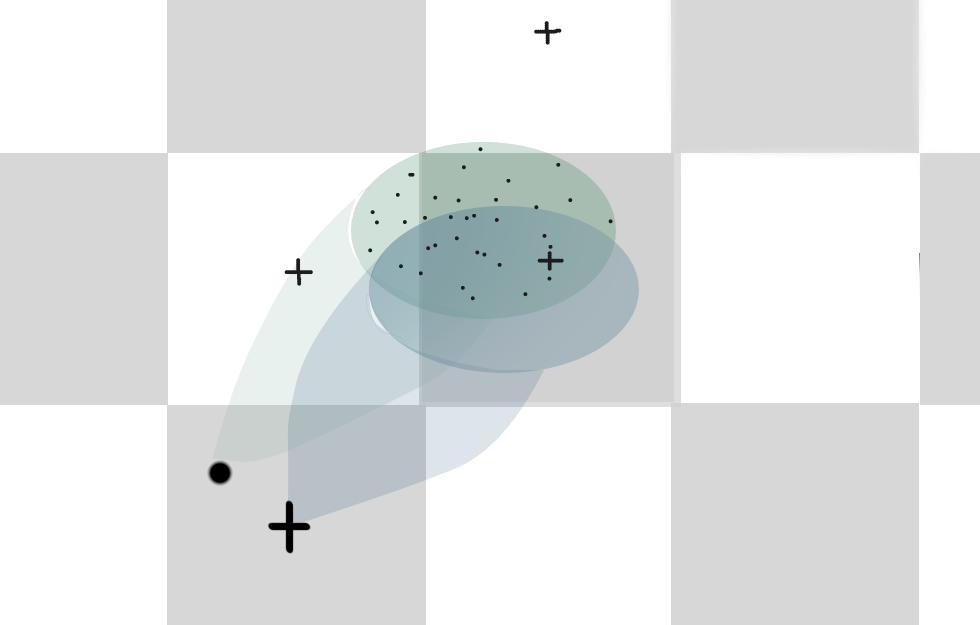
\includegraphics[width = .8\columnwidth]{figs/grid}
	\caption{Depiction of the gridded state space.The mean state of the concrete belief MDP $\bullet$ and the  representative state of the abstract MDP $\boldsymbol{+}$ are given together with an illustration of a stochastic transition. }
\end{figure}
 
Consider a simulation relation defined as 
\axx{I am very happy now :))) finally, i see an example of relation...}
	\begin{align}\label{eq:rel}
\rel := \left\{(s,b_k)| (\hat x_{k|k}-x_s)^T M(\hat x_{k|k}-x_s)\leq \eps, \right.\\\qquad\left.  P^-\preceq P_{k|k} \preceq   P^+ \mbox{ with } b_k=(\hat x_{k|k}, P_{k|k} ) \right\},\notag
	\end{align}
\axx{$x_s$ belongs to belief space. So, it has convariance in it. So, you cannot subtract it from $\hat{x}$.}
\axx{should P+ and P- be in the neighborhoood of covariance part of $x_s$ ?}
and an interface 
\[\InF(\hat u, \hat x, \hat x_{\,|\,}):=K( \hat x_{\,|\,} -\hat x)+\hat u\]
\axx{the notation $\hat x_{\,|\,}$ is weired! what does it represent?}
\axx{interface deserve more explanation and intuition. It is a very key equation/example.}\red{Any suggestion?}
for some matrices $M, K,P^+,P^-$.



We can quantify the difference between $\MB$ and $\hat\MB$ via \eqref{eq:rel} by verifying that for all  $(\hat x_k,\hat x_{k|k})\in \rel$ with probability at least $1-\delta$ it holds that $(\hat x_{k+1},\hat x_{k+1|k+1})\in \rel$. 
Consider a choice for the lifted stochastic  transitions  for \eqref{eq:abstract} and \eqref{eq:beliefx2}, \axx{referred equation is shown later in the text} denoted 
	$ \mathbb W_{x}((\hat x_k, \hat x_{k|k})\in \cdot| \hat u_{k-1}, \hat x_{k-1}, \hat x_{k-1|k-1})$, based on the combined stochastic difference equation given as
\axx{I am staring to understand some of the abstract concepts now.}
\begin{align*}
		&&\hat x_{k+1} &=A\hat x_{k} +B\hat u_{k} + \bar P  C^T  \hat{s}_{k+1},\\%\label{eq:abstract3} \\
	&&\hat x_{k+1|k+1}&=A\hat x_{k|k}+Bu_{k}+  \bar P   C^T(  \hat{s}_{k+1}+s^\Delta_{k+1})\notag\\&&&\qquad+\Delta_{k+1}( \hat{s}_{k+1}+ s^\Delta_{k+1})%\label{eq:beliefx3}
\end{align*}
 with $\Delta_k:=(P_{k|k-1}C^T-  \bar P   C^T)$ and with $ \hat{s}_k\sim \CA N (0,\hat{S}_{inv})$ and $ s^\Delta_k\sim  \CA N (0,\  S_k^{-1}-\hat{S}_{inv}). $

\axx{have you defined P-bar ?}

We can now choose the lifted stochastic transition kernel 	$\Wt$ for the concrete belief MDP $\MB$ and the abstracted finite MDP $\hat\MB$ as follows.
Denote $b=(\hat x_{\,|\,}, P)$ and $b_+=(\hat x_{+\,|\,+}, P_+)$, then 	$\Wt$ is computed as 
 \begin{align*}
 &	\Wt((s_+,b_+)\in \cdot\,| \hat u, s ,b)\\&:= \left\{\begin{array}{ll} \mathbb W_{x}((\Delta_{s_+}, \hat x_{+|+})\in \cdot\,|  \hat u,x_s , \hat x_{\,|\,}) &\text{ for }  P_+=f(P)\\
 	0 & \text{ else } \end{array}\right.
 \end{align*}

For this choice of  	$\mathbb W_x$, the difference expression in \eqref{eq:rel} evolves   as 
\begin{align}
 \hat x_{k+1|k+1}-	\hat x_{k+1}=(A+BK)(\hat x_{k|k}-\hat x_{k-1})\qquad \quad\notag\\+  \bar P   C^T s^\Delta_{k+1} +\Delta_{k+1}( \hat{s}_{k+1}+ s^\Delta_{k+1})\label{eq:beliefx2}
\end{align}
 with $\Delta_{k+1}:=(P_{k+1|k}C^T-  \bar P   C^T)$, and with $ \hat{s}_{k+1}\sim \CA N (0,\hat{S}_{inv})$ and $ s^\Delta_{k+1}\sim  \CA N (0,\  S_{k+1}^{-1}-\hat{S}_{inv}). $
For all $ \hat x_{k+1}$, there exists $\mathbf  r \in \prod_n[-\grid ,\grid]$ such that   $\hat x_{k+1}-\mathbf r \in \{x_s| s \in S\}$. Therefore we can write the update of the difference expression as  \begin{align}
 \hat x_{+|+}-	\hat x_{s_+}=(A+BK)(\hat x_{\,|\,}-\hat x_s)+\mathbf r\qquad \quad\notag\\+  \bar P   C^T s^\Delta_{k+1} +\Delta_{k+1}( \hat{s}_{k+1}+ s^\Delta_{k+1})\label{eq:beliefx2}.
\end{align}
Given that $(\hat x_{\,|\,}-\hat x_s)$ and  $\mathbf r$ belongs to a bounded set, we can bound the influence of the noise terms $s^\Delta_{k+1}$ and $ \hat{s}_{k+1}$ with respect to a probability at least $1-\delta$ for which the update is always in $\rel$ see equation \eqref{eq:rel}.


\new{More precisely, compute a lower bound on \begin{align}
&\po\left((A+BK)(\hat x_{\,|\,}-\hat x_s)+\mathbf r\qquad \quad\notag\right.\\&\left.+  \bar P   C^T s^\Delta_{k+1} + \Delta_{k+1} s^\Delta_{k+1}+\Delta_{k+1} \hat{s}_{k+1} \in \rel\right)\label{eq:condition1}
\end{align}
given that $(\hat x_{\,|\,},\hat x_s)\in \rel$.  
Given bounded sets $X_\Delta$, $\hat C_\Delta$, and  $C_\Delta$, we replace the probability condition \eqref{eq:condition1} with  
\begin{align}
&  (A+BK)x_\delta+\mathbf r  + c_{\Delta} +\hat c_{\Delta} \in \rel 
\end{align}
for all $x_\Delta\in X_\Delta :=\{(\hat x_{\,|\,}-\hat x_s)\in \rel\}$, $\hat c_{\Delta} \in \hat C_\Delta$ and for all $ c_{\Delta} \in  C_\Delta$.
 
}



%    
%Consider the linear time invariant system with Gaussian disturbance, given as 
%\begin{align}\begin{aligned}
%	x^m_{k+1} &= A x^m_{k}+B^mu_{k}+ F^m w_{k}\\
%	y^m_{k}&=C^m x^m_{k}+D^m u_{k}+E^m v_{k}\end{aligned}
%\end{align}
%with matrices $A,B,C,D$ and matrices $F,E$. 
%The measurement noise signal $v$ is zero-mean, independently and identically  distributed noise, i.e, $v_k\sim \mathcal{N}(0,I)$.
%% \noindent\textbf{Wind disturbance.}
%The state transitions are affected by the wind $w_k$. 
%We can model the dynamic variations of the wind as filtered noise. 
%There are two commonly used models  \citep{richardson2013quantifying},  this includes the von Karman power spectral density,
%and the Dryden model.
%The former model matches experiment data more than the 
% Dryden model, but the Dryden model can be represented by  a lower order filter.
%Consider a filter model to be given as
%\begin{align}
%	\begin{aligned}
%	x_{t+1}^w &= A^w x_{t}^w+ F^w e_{t},\\
%	w_{t}&=C^w x_{t}^w+E^w e_{t}.
%	\end{aligned}
%\end{align}
%
%%\textbf{Full model \& Belief space model.}
%The full model is given as follows
%%\begin{align} 
%%	\begin{bmatrix}
%%	x^m_{t+1}	\\x^w_{t+1}
%%	\end{bmatrix}
%% &= \begin{bmatrix}
%% 	A^m 	& F^mC^w\\
%% 	0 & A^w
%% \end{bmatrix}
%%\begin{bmatrix}
%%	x^m_{t}	\\x^w_{t}
%%	\end{bmatrix}+\begin{bmatrix} B^m \\ 0~ \end{bmatrix} u_{t}+  \begin{bmatrix}
%%	F^m E^w \\
%%	F^w
%%	\end{bmatrix}e_{t}\notag\\
%%	y^m_{t}&=\begin{bmatrix} C^m& 0 \end{bmatrix}\begin{bmatrix}
%%	x^m_{t}	\\x^w_{t}
%%	\end{bmatrix}+D^m u_{t}+E^m v_{t}.
%%\end{align}
%%This can be written as 
% \begin{align}  \begin{aligned}
%x_{t+1}&=A x_{t} + B u_t+ Fe_t\\
%y_t&=Cx_t+Du_t+Ev_t\end{aligned} \end{align}
%\begin{align}& \mbox{ with }  x_t	= \begin{bmatrix}
%	x^m_{t}	\\x^w_{t}
%	\end{bmatrix},
%A = \begin{bsmallmatrix}
% 	A^m 	& F^mC^w\\
% 	0 & A^w
% \end{bsmallmatrix}\!, \ 
%B = \begin{bsmallmatrix} B^m \\ 0~ \end{bsmallmatrix}\!,\notag \\
%&F=\begin{bsmallmatrix}
%	F^m E^w \\
%	F^w
%	\end{bsmallmatrix}\!,\ 
%C = \begin{bmatrix} C^m& 0 \end{bmatrix}\!, \ 
%D= D^m, \  E = E^m.\notag
%\end{align}
% 
% \noindent{\textbf{}}
%
%    
  
    
    \section{Case study}
    %!TEX root = 3_FormalAbstraction inLTLUnderUncertainty.tex

Motivated by space exploration applications, we consider an autonomous rover tasked with identifying and collecting scientific samples.


\textbf{Rover model.} Without loss of generality, we consider a simple rover model as a point mass $x_k \in \mathbb{R}^2$ affected by stochastic disturbances. We also assume that the position of the rover cannot be measured exactly and model its dynamics as
\begin{equation*}
\begin{aligned}
	x_{k+1}&= x_{k} + u_k+ w_k,  & w_k \sim \CA N \left(0,\begin{bmatrix}.4&-.2\\-.2&.4\end{bmatrix}\right), \\
	z_k&= x_k+v_k, &  v_k \sim \CA N \left(0,\begin{bmatrix}1&.1\\.1&1\end{bmatrix}\right).
\end{aligned}
\end{equation*}

A finite abstraction $\MDP_{syst}$ is constructed as outlined in the previous section by discretizing the state space $[-10, 10]^2$ with a discretization parameter $\grid = (0.76481, 0.64426)$, and by representing the input space $[-1,1]^2$ with nine discrete inputs $\{0, 1, -1\}^2$.

\begin{figure}
	% This file was created by matplotlib2tikz v0.6.14.
\centering
\begin{tikzpicture}
\newlength\figurewidth
\newlength\figureheight
\setlength\figurewidth{\columnwidth}
\setlength\figureheight{.4\columnwidth}
\definecolor{color0}{rgb}{0.12156862745098,0.466666666666667,0.705882352941177}

\begin{axis}[scale =.8,
xlabel={$\delta$},
ylabel={$\epsilon$},
xmin=-0.01395, xmax=0.25,
ymin=0.8, ymax=1.45222764450879,
width=\figurewidth,
height=\figureheight,
% tick align=outside,
% tick pos=left,
x grid style={lightgray!92.026143790849673!black},
y grid style={lightgray!92.026143790849673!black},
axis y line=left,
axis x line=middle,
every axis x label/.style={
    at={(ticklabel* cs:1.05)}
}
]
\addplot [semithick, color0, forget plot,  mark=*,mark options={scale=.84}]
table {%
0.001 1.4272384844875
0.0167368421052632 1.22339465219428
0.0324736842105263 1.16617411196529
0.0482105263157895 1.13191279574885
0.0639473684210526 1.10601589042324
0.0796842105263158 1.08400668945514
0.0954210526315789 1.06721503359466
0.111157894736842 1.05265893349788
0.126894736842105 1.04157018327801
0.142631578947368 1.02417176675944
0.158368421052632 1.01254639660019
0.174105263157895 1.00120158889137
0.189842105263158 0.991557539021032
0.205578947368421 0.982277989301703
0.221315789473684 0.97353496742902
0.237052631578947 0.965239656823681
0.252789473684211 0.960158902624749
0.268526315789474 0.951512372393061
0.284263157894737 0.927455284061691
0.3 0.935781247731614
};
\end{axis}

\end{tikzpicture}
	\caption{Trade-off between $\epsilon$ and $\delta$.  }
\end{figure}

\textbf{Environment model.} We consider sample collection in a partially unknown environment. In particular, there are two potential target regions $T_1$ and $T_2$ where the probability of encountering a sample has been assessed via satellite imagery as 0.5 and 0.6, respectively. In addition, there are two potential obstacle regions $O_1$ and $O_2$ where estimates give probabilities of 0.9 and 0.7 that the rover can traverse the area safely. For both target and obstacle regions, we assume that the true nature of the region can be determined when the rover is within a certain distance of the regions. The regions are illustrated in Figs. \ref{fig:exp1} and \ref{fig:exp2}.

The dynamics of the uncertainty in $T_1$ can be modeled as an MDP with three states \texttt{init}, \texttt{sample} and \texttt{empty}, and two actions \texttt{measure} and \texttt{none}. Initially, the state is \texttt{init}. If the \texttt{measure} action is performed, the state transitions to \texttt{sample} with probability $p$ and to \texttt{empty} with probability $1-p$. After a measurement, no further transitions occur. This type of MDP can be constructed for each region of uncertainty, and the overall environment model $\MDP_{env}$ is their parallel composition. \red{Furthermore, we model a failure probability of 0.01 at each step with an additional MDP $\MDP_{fail}$ which discourages solutions that take long time to execute.}

\textbf{Specification.} The objective is to collect a sample while avoiding unsafe regions. To this end, we consider the scLTL specification
\begin{equation}
	\psi = \lozenge \texttt{sample} \land \left( \lnot \texttt{fail} \; \mathcal {U} \; \texttt{sample} \right),
\end{equation}
where the atomic proposition \texttt{sample} is true if the rover is in a target region that has been determined to contain a sample, and the atomic proposition \texttt{fail} is defined as being true if 1) the rover is in an obstacle region that contains an obstacle, or 2) $\MDP_{fail}$ is in failure mode.

\textbf{Results.} We consider the aggregate system $\MDP_{syst} \times \MDP_{env} \times \MDP_{fail}$ defined as a product system analogous to Definition \ref{def:product}, which is an MDP with 9 inputs and 277182 states. Via \eqref{eq:prob:robust_optimal} we synthesize a control policy that is robust to the difference between the concrete and abstract models. Figs. \ref{fig:exp1} and \ref{fig:exp2} depict the evolution of the estimated position for executions generated by the control policies, and the estimated probability that the specification can be satisfied, under two different resolutions of the unknown environment. In both experiments only $T_2$ contains a sample, and $O_1$ contains an obstacle. The difference is that in Fig. \ref{fig:exp1} also $O_2$ turns out to contain an obstacle but in Fig. \ref{fig:exp2} this region can be safely traversed.

\begin{figure}
	\footnotesize
	\setlength\figurewidth{\columnwidth} 
	\setlength\figureheight{0.6\columnwidth} 

	% This file was created by matplotlib2tikz v0.6.14.
\begin{tikzpicture}

\definecolor{color1}{rgb}{1,0.498039215686275,0.0549019607843137}
\definecolor{color0}{rgb}{0.12156862745098,0.466666666666667,0.705882352941177}
\definecolor{color3}{rgb}{0.83921568627451,0.152941176470588,0.156862745098039}
\definecolor{color2}{rgb}{0.172549019607843,0.627450980392157,0.172549019607843}
\definecolor{color5}{rgb}{0.549019607843137,0.337254901960784,0.294117647058824}
\definecolor{color4}{rgb}{0.580392156862745,0.403921568627451,0.741176470588235}

\begin{axis}[
xlabel={$x_1$},
ylabel={$x_2$},
xmin=-11.1088588047251, xmax=11.1145664581499,
ymin=-10.1108621762447, ymax=10.9576601036307,
width=\figurewidth,
height=\figureheight,
tick align=outside,
tick pos=left,
mark size=1,
x grid style={lightgray!92.026143790849673!black},
y grid style={lightgray!92.026143790849673!black}
]
\addplot [only marks, draw=black, fill=black, colormap/viridis]
table{%
x                      y
-1.000000000000000e+01 -9.000000000000000e+00
-8.869595294321220e+00 -7.814207719224903e+00
-7.104778400743559e+00 -7.140354399223419e+00
-6.376752541526766e+00 -6.870554896721502e+00
-4.832702844468539e+00 -6.036032413666041e+00
-4.377547654253716e+00 -5.216915548266608e+00
-3.744230908366174e+00 -3.905880113729608e+00
-2.871984978581734e+00 -2.567990703687725e+00
-3.127375571989979e+00 -2.090610019084363e+00
-2.305771899885637e+00 -9.338180566109633e-01
-3.687373068419801e+00 +4.769618066414293e-01
-4.131753222593663e+00 +9.557682476343059e-01
-4.601633165510158e+00 +1.661042239367786e+00
-5.694730614871723e+00 +4.003513878529873e+00
-5.973575212285128e+00 +3.578554273124150e+00
-6.299886148045688e+00 +3.044114991420233e+00
-4.771656903671562e+00 +2.858962077904698e+00
-4.543639365229525e+00 +2.139567825321754e+00
-2.673138926724003e+00 +1.798961623791945e+00
-3.527414786094551e+00 +3.231833707854521e+00
-2.124252800165384e+00 +2.332430078604584e+00
-1.336517727306551e+00 +1.867196593378676e+00
-1.601443252054275e+00 +2.126202270702624e+00
-2.276211315148957e+00 +3.308254449757351e+00
-7.301645225187249e-01 +4.522420844572547e+00
+6.421309072702257e-01 +5.679192620151055e+00
+6.291550303486995e-01 +6.527896371328548e+00
+1.619950872445812e+00 +7.559823424104585e+00
+3.103218944956174e+00 +6.190024650395538e+00
+5.076329139729479e+00 +6.568676876712611e+00
+5.892120984615905e+00 +7.942903477538653e+00
+5.647060738990990e+00 +8.410805253485940e+00
+6.378542919870930e+00 +7.216198212323969e+00
+5.911651447016797e+00 +6.074808626739333e+00
};
\addplot [only marks, draw=black, fill=black, colormap/viridis]
table{%
x                      y
-6.000000000000000e+00 -9.000000000000000e+00
-5.901406929599968e+00 -7.508199438071110e+00
-4.358884763233826e+00 -5.792082591551480e+00
-3.919800671528496e+00 -4.077694923566842e+00
-3.692867013779527e+00 -2.339134536400095e+00
-4.122397810293728e+00 -8.975301878708711e-01
-2.490405176513862e+00 -2.573953379208296e-01
-4.111781121286302e+00 +1.145086563115543e+00
-3.677892980298973e+00 +1.377137896197289e+00
-3.566602837148350e+00 +8.815148406364688e-01
-3.338101562637621e+00 +1.932094838504950e+00
-4.516623627187172e+00 +2.134782889471700e+00
-5.049009747014780e+00 +3.556356142323278e+00
-5.015975542724512e+00 +4.642632272866249e+00
-4.249031141395299e+00 +3.638868112650753e+00
-3.606475659338956e+00 +3.327243509372837e+00
-2.389126541991601e+00 +2.001450651124150e+00
-1.783057348634495e+00 +1.573015875488078e+00
-2.981625704030834e+00 +3.183156711833124e+00
-2.358357517805116e+00 +4.479839517723944e+00
-2.288659157327666e+00 +6.279107959374064e+00
-1.411436975902111e+00 +6.189266978612975e+00
-5.320073996643725e-01 +6.157716555765220e+00
-5.104133024329928e-01 +7.405451568002405e+00
+1.274177610274697e+00 +5.346446814476317e+00
+3.328125868896929e+00 +5.848995543358567e+00
+3.432597856511344e+00 +7.459258972502006e+00
+4.030094855910188e+00 +7.728847292266309e+00
+5.354424702892910e+00 +8.500182463536220e+00
+6.155873129399546e+00 +6.918829831869020e+00
+5.925808542673061e+00 +6.475595415762200e+00
};
\addplot [only marks, draw=black, fill=black, colormap/viridis]
table{%
x                      y
-2.000000000000000e+00 -9.000000000000000e+00
-3.044462714452268e+00 -7.306350162100894e+00
-2.293090798054657e+00 -7.301138964922043e+00
-2.992445270727864e+00 -5.860237642906498e+00
-2.700570628355699e+00 -5.891003937213707e+00
-3.261421640643176e+00 -4.215783895557847e+00
-3.158411977295807e+00 -2.780961678014854e+00
-3.143450533987836e+00 -2.507508068387384e+00
-3.025567040118594e+00 -2.323985887674691e+00
-3.147878570292180e+00 -1.765176888234320e+00
-3.321097798094850e+00 -8.960733607114131e-01
-3.071809481398453e+00 +2.656018153234110e-01
-3.347289674472285e+00 +2.525143550310250e+00
-4.343077763169791e+00 +3.655246402097009e+00
-4.746507006214285e+00 +4.694914521302897e+00
-4.773216787388434e+00 +4.346197557892083e+00
-4.295952786822955e+00 +3.660497376626418e+00
-3.143953286965482e+00 +2.625049791199087e+00
-1.641162836868084e+00 +2.688373056222609e+00
-2.041754565063155e+00 +2.649157162515526e+00
-3.306752490703531e+00 +3.253350556635815e+00
-2.983336851770111e+00 +3.971825313172622e+00
-2.469010596282821e+00 +4.546595568617136e+00
-1.228788797359903e+00 +5.627707538998200e+00
-1.094952620493618e+00 +8.175427155795038e+00
-9.592574172669480e-01 +8.082721342294306e+00
-1.194386354456936e+00 +8.165264896530068e+00
-4.616822792871155e-01 +6.621700444105216e+00
+7.497631277014686e-01 +7.076610441120152e+00
+1.979746828542337e+00 +6.612237335050672e+00
+3.128826364302311e+00 +6.253528797214032e+00
+4.025272616622998e+00 +6.503242452969750e+00
+3.645362150228443e+00 +7.636106778389254e+00
+5.261846571766094e+00 +6.237023538647955e+00
+5.641826018152110e+00 +7.725113353647728e+00
+6.812612257678752e+00 +7.585618827435113e+00
+6.232989074320007e+00 +8.719742643797003e+00
};
\addplot [only marks, draw=black, fill=black, colormap/viridis]
table{%
x                      y
+2.000000000000000e+00 -9.000000000000000e+00
+2.952866870372958e+00 -8.576100227432466e+00
+4.242197553383458e+00 -7.804545716747594e+00
+5.074855341092752e+00 -5.625352120055734e+00
+4.830608053317017e+00 -5.307135825638624e+00
+6.260668707794887e+00 -4.393024727214535e+00
+5.626132234535231e+00 -3.468882934108938e+00
+4.360920432033688e+00 -1.633814410374898e+00
+5.283892683157318e+00 -9.239872896419613e-01
+6.137055506057617e+00 -2.713402990434055e-01
+3.960819582615776e+00 +7.198393840378496e-01
+4.348495153676051e+00 +2.182925104805387e+00
+5.310490549051644e+00 +3.346073054040058e+00
+5.927805236978374e+00 +3.532146335797724e+00
+7.076206486765265e+00 +4.595056538443954e+00
+6.905541839334503e+00 +6.818868569963236e+00
+6.916859672204205e+00 +6.538704789396275e+00
};
\addplot [only marks, draw=black, fill=black, colormap/viridis]
table{%
x                      y
+6.000000000000000e+00 -9.000000000000000e+00
+7.656026307682226e+00 -7.552110273740422e+00
+6.106733751763857e+00 -4.944778792524008e+00
+5.007607308637190e+00 -4.476890270578113e+00
+5.340307715623565e+00 -3.870524755975019e+00
+5.223674090042989e+00 -2.999138613814250e+00
+4.852825372926093e+00 -1.649771429171313e+00
+5.277460910519775e+00 -6.637444320456167e-01
+3.912214555867033e+00 +4.809921810937652e-01
+4.689101241974543e+00 +1.514074549520304e+00
+5.988818016236550e+00 +1.998528533661037e+00
+5.506348480377154e+00 +3.663415125077347e+00
+5.339192804183695e+00 +4.558762439747721e+00
+7.256112587009863e+00 +5.131362769874022e+00
+7.631959808780144e+00 +5.683576842740282e+00
+7.257947121647226e+00 +7.090711607035485e+00
+6.414874444391497e+00 +6.824546651611620e+00
};
\addplot [only marks, draw=black, fill=black, colormap/viridis]
table{%
x                      y
+1.000000000000000e+01 -9.000000000000000e+00
+8.501744459872617e+00 -7.514163496353530e+00
+7.502543301317530e+00 -6.247529485824156e+00
+6.789481505237688e+00 -5.327060783448672e+00
+6.299648866376312e+00 -4.120122662433571e+00
+4.477615169608585e+00 -3.392450768338643e+00
+5.941939396771113e+00 -2.155271399521218e+00
+4.924919113275441e+00 -1.405474597240854e+00
+4.038299633666932e+00 -2.035680327253797e-01
+5.189304536388701e+00 +1.018679026545901e+00
+4.395910542655945e+00 +2.158524989021073e+00
+6.551109435674287e+00 +2.948566939226978e+00
+6.949044679173154e+00 +3.493783802114474e+00
+4.470283883624948e+00 +5.678295462897534e+00
+7.557669000755279e+00 +6.353439694488499e+00
+7.116516078033896e+00 +6.021511860498869e+00
};
\path [draw=red, fill=red, opacity=0.5] (axis cs:2,-5)
--(axis cs:2,2)
--(axis cs:0,2)
--(axis cs:0,-5)
--cycle;

\path [draw=red, fill=red, opacity=0.5] (axis cs:2,3)
--(axis cs:2,10)
--(axis cs:0,10)
--(axis cs:0,3)
--cycle;

\path [draw=blue, fill=blue, opacity=0.5] (axis cs:-6,6)
--(axis cs:-6,9)
--(axis cs:-9,9)
--(axis cs:-9,6)
--cycle;

\path [draw=blue, fill=blue, opacity=0.5] (axis cs:9,6)
--(axis cs:9,9)
--(axis cs:6,9)
--(axis cs:6,6)
--cycle;

\addplot [semithick, color0, forget plot]
table {%
-10 -9
-8.86959529432122 -7.8142077192249
-7.10477840074356 -7.14035439922342
-6.37675254152677 -6.8705548967215
-4.83270284446854 -6.03603241366604
-4.37754765425372 -5.21691554826661
-3.74423090836617 -3.90588011372961
-2.87198497858173 -2.56799070368773
-3.12737557198998 -2.09061001908436
-2.30577189988564 -0.933818056610963
-3.6873730684198 0.476961806641429
-4.13175322259366 0.955768247634306
-4.60163316551016 1.66104223936779
-5.69473061487172 4.00351387852987
-5.97357521228513 3.57855427312415
-6.29988614804569 3.04411499142023
-4.77165690367156 2.8589620779047
-4.54363936522953 2.13956782532175
-2.673138926724 1.79896162379194
-3.52741478609455 3.23183370785452
-2.12425280016538 2.33243007860458
-1.33651772730655 1.86719659337868
-1.60144325205428 2.12620227070262
-2.27621131514896 3.30825444975735
-0.730164522518725 4.52242084457255
0.642130907270226 5.67919262015106
0.629155030348699 6.52789637132855
1.61995087244581 7.55982342410458
3.10321894495617 6.19002465039554
5.07632913972948 6.56867687671261
5.8921209846159 7.94290347753865
5.64706073899099 8.41080525348594
6.37854291987093 7.21619821232397
5.9116514470168 6.07480862673933
};
\addplot [semithick, color1, forget plot]
table {%
-6 -9
-5.90140692959997 -7.50819943807111
-4.35888476323383 -5.79208259155148
-3.9198006715285 -4.07769492356684
-3.69286701377953 -2.3391345364001
-4.12239781029373 -0.897530187870871
-2.49040517651386 -0.25739533792083
-4.1117811212863 1.14508656311554
-3.67789298029897 1.37713789619729
-3.56660283714835 0.881514840636469
-3.33810156263762 1.93209483850495
-4.51662362718717 2.1347828894717
-5.04900974701478 3.55635614232328
-5.01597554272451 4.64263227286625
-4.2490311413953 3.63886811265075
-3.60647565933896 3.32724350937284
-2.3891265419916 2.00145065112415
-1.7830573486345 1.57301587548808
-2.98162570403083 3.18315671183312
-2.35835751780512 4.47983951772394
-2.28865915732767 6.27910795937406
-1.41143697590211 6.18926697861298
-0.532007399664372 6.15771655576522
-0.510413302432993 7.40545156800241
1.2741776102747 5.34644681447632
3.32812586889693 5.84899554335857
3.43259785651134 7.45925897250201
4.03009485591019 7.72884729226631
5.35442470289291 8.50018246353622
6.15587312939955 6.91882983186902
5.92580854267306 6.4755954157622
};
\addplot [semithick, color2, forget plot]
table {%
-2 -9
-3.04446271445227 -7.30635016210089
-2.29309079805466 -7.30113896492204
-2.99244527072786 -5.8602376429065
-2.7005706283557 -5.89100393721371
-3.26142164064318 -4.21578389555785
-3.15841197729581 -2.78096167801485
-3.14345053398784 -2.50750806838738
-3.02556704011859 -2.32398588767469
-3.14787857029218 -1.76517688823432
-3.32109779809485 -0.896073360711413
-3.07180948139845 0.265601815323411
-3.34728967447229 2.52514355031025
-4.34307776316979 3.65524640209701
-4.74650700621429 4.6949145213029
-4.77321678738843 4.34619755789208
-4.29595278682296 3.66049737662642
-3.14395328696548 2.62504979119909
-1.64116283686808 2.68837305622261
-2.04175456506316 2.64915716251553
-3.30675249070353 3.25335055663581
-2.98333685177011 3.97182531317262
-2.46901059628282 4.54659556861714
-1.2287887973599 5.6277075389982
-1.09495262049362 8.17542715579504
-0.959257417266948 8.08272134229431
-1.19438635445694 8.16526489653007
-0.461682279287116 6.62170044410522
0.749763127701469 7.07661044112015
1.97974682854234 6.61223733505067
3.12882636430231 6.25352879721403
4.025272616623 6.50324245296975
3.64536215022844 7.63610677838925
5.26184657176609 6.23702353864796
5.64182601815211 7.72511335364773
6.81261225767875 7.58561882743511
6.23298907432001 8.719742643797
};
\addplot [semithick, color3, forget plot]
table {%
2 -9
2.95286687037296 -8.57610022743247
4.24219755338346 -7.80454571674759
5.07485534109275 -5.62535212005573
4.83060805331702 -5.30713582563862
6.26066870779489 -4.39302472721454
5.62613223453523 -3.46888293410894
4.36092043203369 -1.6338144103749
5.28389268315732 -0.923987289641961
6.13705550605762 -0.271340299043406
3.96081958261578 0.71983938403785
4.34849515367605 2.18292510480539
5.31049054905164 3.34607305404006
5.92780523697837 3.53214633579772
7.07620648676526 4.59505653844395
6.9055418393345 6.81886856996324
6.9168596722042 6.53870478939627
};
\addplot [semithick, color4, forget plot]
table {%
6 -9
7.65602630768223 -7.55211027374042
6.10673375176386 -4.94477879252401
5.00760730863719 -4.47689027057811
5.34030771562356 -3.87052475597502
5.22367409004299 -2.99913861381425
4.85282537292609 -1.64977142917131
5.27746091051977 -0.663744432045617
3.91221455586703 0.480992181093765
4.68910124197454 1.5140745495203
5.98881801623655 1.99852853366104
5.50634848037715 3.66341512507735
5.3391928041837 4.55876243974772
7.25611258700986 5.13136276987402
7.63195980878014 5.68357684274028
7.25794712164723 7.09071160703548
6.4148744443915 6.82454665161162
};
\addplot [semithick, color5, forget plot]
table {%
10 -9
8.50174445987262 -7.51416349635353
7.50254330131753 -6.24752948582416
6.78948150523769 -5.32706078344867
6.29964886637631 -4.12012266243357
4.47761516960859 -3.39245076833864
5.94193939677111 -2.15527139952122
4.92491911327544 -1.40547459724085
4.03829963366693 -0.20356803272538
5.1893045363887 1.0186790265459
4.39591054265594 2.15852498902107
6.55110943567429 2.94856693922698
6.94904467917315 3.49378380211447
4.47028388362495 5.67829546289753
7.55766900075528 6.3534396944885
7.1165160780339 6.02151186049887
};
\node at (axis cs:1,1)[
  scale=0.5,
  anchor=base west,
  text=black,
  rotate=0.0
]{ $O_1$};
\node at (axis cs:1,9)[
  scale=0.5,
  anchor=base west,
  text=black,
  rotate=0.0
]{ $O_2$};
\node at (axis cs:-9,8)[
  scale=0.5,
  anchor=base west,
  text=black,
  rotate=0.0
]{ $T_1$};
\node at (axis cs:8,8)[
  scale=0.5,
  anchor=base west,
  text=black,
  rotate=0.0
]{ $T_2$};
\end{axis}

\end{tikzpicture}
	\setlength\figureheight{0.4\columnwidth} 

	% This file was created by matplotlib2tikz v0.6.14.
\begin{tikzpicture}

\definecolor{color1}{rgb}{1,0.498039215686275,0.0549019607843137}
\definecolor{color0}{rgb}{0.12156862745098,0.466666666666667,0.705882352941177}
\definecolor{color3}{rgb}{0.83921568627451,0.152941176470588,0.156862745098039}
\definecolor{color2}{rgb}{0.172549019607843,0.627450980392157,0.172549019607843}
\definecolor{color5}{rgb}{0.549019607843137,0.337254901960784,0.294117647058824}
\definecolor{color4}{rgb}{0.580392156862745,0.403921568627451,0.741176470588235}

\begin{axis}[
xlabel={$t$},
ylabel={$\mathbb{P}(\varphi)$},
xmin=-1.8, xmax=37.8,
ymin=0.38853456067633, ymax=1.02911740187259,
width=\figurewidth,
height=\figureheight,
tick align=outside,
tick pos=left,
x grid style={lightgray!92.026143790849673!black},
y grid style={lightgray!92.026143790849673!black}
]
\addplot [semithick, color0, forget plot]
table {%
0 0.566291945691099
1 0.566291945691099
2 0.605882976959095
3 0.612354132971019
4 0.615146535917152
5 0.620313388350838
6 0.623169341037894
7 0.632266923722546
8 0.640795190330476
9 0.64428856744584
10 0.650176429635556
11 0.660779548866506
12 0.664373678411201
13 0.667953572290617
14 0.421487160337076
15 0.419564608493884
16 0.417651962548887
17 0.424169566255033
18 0.426345484650421
19 0.431108756242508
20 0.430751120445197
21 0.433029533909929
22 0.436207218324974
23 0.436207218324974
24 0.448504360104309
25 0.462109503911388
26 0.466372172152465
27 0.468495540003818
28 0.474972821467856
29 0.480216364807438
30 0.979868029536619
31 0.988089397434187
32 0.983895865110246
33 1.00000000000003
};
\addplot [semithick, color1, forget plot]
table {%
0 0.598873106893363
1 0.598873106893363
2 0.611938797531012
3 0.620313388350838
4 0.632266923722546
5 0.641338529177884
6 0.651286575651904
7 0.653667661427169
8 0.664373678411201
9 0.667389245077004
10 0.663807726695736
11 0.670472509073791
12 0.671058796741362
13 0.680876876002895
14 0.423299602729996
15 0.428005120445258
16 0.430751120445197
17 0.431108756242508
18 0.436564779737749
19 0.448714044552832
20 0.455361601380584
21 0.454662990626655
22 0.459229983640598
23 0.463841336213989
24 0.463444874596063
25 0.471062027085172
26 0.482793941967823
27 0.479801326577619
28 0.969453775583137
29 0.983895865110246
30 1.00000000000003
};
\addplot [semithick, color2, forget plot]
table {%
0 0.601199049439663
1 0.601199049439663
2 0.611373258769312
3 0.610825977206025
4 0.61950569968835
5 0.61950569968835
6 0.628810791270583
7 0.637985226843664
8 0.641338529177884
9 0.64428856744584
10 0.64428856744584
11 0.65073129659484
12 0.657238925992285
13 0.673118973708607
14 0.680502261669169
15 0.423299602729996
16 0.425630605759241
17 0.428005120445258
18 0.432928711351226
19 0.444768945274215
20 0.442429168485533
21 0.445763301335716
22 0.452612154776499
23 0.455361601380584
24 0.459622816160484
25 0.458418097195606
26 0.460938662424354
27 0.458418097195606
28 0.461333021386082
29 0.468094526343635
30 0.475377924614331
31 0.480216364807438
32 0.970297252430312
33 0.963929119062114
34 0.979868029536619
35 0.984943443987629
36 1.00000000000003
};
\addplot [semithick, color3, forget plot]
table {%
0 0.60221316758681
1 0.60221316758681
2 0.603095656982768
3 0.612754055717539
4 0.624538495801648
5 0.62791668893401
6 0.633081343456916
7 0.639922816020793
8 0.646852485781285
9 0.652756759496805
10 0.658726606328146
11 0.655977449212481
12 0.665293062315518
13 0.671265524930602
14 0.673823637438148
15 0.974478764836217
16 1.00000000000003
};
\addplot [semithick, color4, forget plot]
table {%
0 0.601395515122941
1 0.601395515122941
2 0.61392554430982
3 0.630267741952442
4 0.630807082939585
5 0.633670305343681
6 0.639922816020793
7 0.649819559965179
8 0.659285200283324
9 0.652182261074434
10 0.658796362546444
11 0.661342844708322
12 0.673823637438148
13 0.969766480712513
14 0.979000636609888
15 0.984943431279268
16 1.00000000000003
};
\addplot [semithick, color5, forget plot]
table {%
0 0.511047337255817
1 0.511047337255817
2 0.612978700250407
3 0.620063167202848
4 0.626830204231395
5 0.633081343456916
6 0.640464676396021
7 0.649268206152165
8 0.649819559965179
9 0.659844019602223
10 0.665920200487818
11 0.67605034228333
12 0.681786379389656
13 0.684269702304902
14 0.974797775257462
15 1.00000000000003
};
\end{axis}

\end{tikzpicture}
	\caption{Above: six trajectories starting at different initial conditions. Below: estimated probability to satisfy the specification over time for the same trajectories. No sample is found in $T_1$, and $O_2$ can be safely traversed. Jumps occur in the probabilities when (non-)existence of samples are measured when the rover is close to the regions.}
	\label{fig:exp1}
\end{figure}

\begin{figure}
	\footnotesize
	\setlength\figurewidth{\columnwidth} 
	\setlength\figureheight{0.6\columnwidth} 

	% This file was created by matplotlib2tikz v0.6.14.
\begin{tikzpicture}

\definecolor{color1}{rgb}{1,0.498039215686275,0.0549019607843137}
\definecolor{color0}{rgb}{0.12156862745098,0.466666666666667,0.705882352941177}
\definecolor{color2}{rgb}{0.172549019607843,0.627450980392157,0.172549019607843}

\begin{axis}[
mark size = 0.5,
ticks=none,
xmin=-11, xmax=11,
ymin=-10.6290882408405, ymax=10.9823375352781,
width=\figurewidth,
height=\figureheight,
tick align=outside,
tick pos=left,
x grid style={lightgray!92.026143790849673!black},
y grid style={lightgray!92.026143790849673!black}
]
\addplot [only marks, draw=black, fill=black, colormap/viridis]
table{%
x                      y
-8.000000000000000e+00 -9.000000000000000e+00
-8.281791193811282e+00 -6.953277059756937e+00
-6.609947231673338e+00 -7.304755895777043e+00
-6.447420151999264e+00 -6.984253859219061e+00
-5.930025319876885e+00 -6.296279125763103e+00
-5.476123458484502e+00 -6.049868453584115e+00
-4.680375628377898e+00 -4.982516422756326e+00
-3.356608221836718e+00 -4.767445283086258e+00
-3.850337386959414e+00 -3.882953851781119e+00
-3.888519145722516e+00 -3.480146659512000e+00
-5.320305970691908e+00 -2.277119535242806e+00
-4.379722627893722e+00 -3.023297381626749e+00
-2.966831046751209e+00 -2.008805754832921e+00
-4.696058526749306e+00 +1.019091306738935e-01
-4.628219306657023e+00 +1.300100090541606e+00
-5.641564937919985e+00 +1.796635145522380e+00
-6.307184225641461e+00 +2.288130625455808e+00
-7.217828733789983e+00 +3.143921812081298e+00
-7.301911031188013e+00 +4.255956608402649e+00
-6.401344954223192e+00 +5.270680166902547e+00
-8.171856419882948e+00 +6.563080734161627e+00
};
\addplot [only marks, draw=black, fill=black, colormap/viridis]
table{%
x                      y
+0.000000000000000e+00 -9.000000000000000e+00
+2.985780663708160e-02 -8.155463278156050e+00
+1.071409254737555e+00 -8.202590105544974e+00
+2.130577217930679e+00 -8.147034783291767e+00
+3.046653997506764e+00 -7.814782310273142e+00
+2.993503950729483e+00 -6.732513426782055e+00
+3.364980364937721e+00 -5.919601911047740e+00
+4.577267269183741e+00 -5.442531058948178e+00
+4.641924364448064e+00 -4.277469389688367e+00
+4.066522550812240e+00 -2.261074508296681e+00
+4.900884132823337e+00 -1.747839224197387e+00
+5.242948546817824e+00 -1.658932790996334e+00
+4.951650027020797e+00 -5.458682191996835e-01
+5.160727075484108e+00 +1.786499818804027e-02
+4.951600531141041e+00 +3.796585040088380e-01
+5.548111410812709e+00 +9.093914656273301e-01
+5.998289710281483e+00 +1.845859092339620e+00
+5.586468819814069e+00 +2.958893844938457e+00
+6.773322394657046e+00 +4.341573264475908e+00
+6.244801362810740e+00 +3.255339248138667e+00
+5.386058184710604e+00 +2.832977405694789e+00
+3.382447161292124e+00 +5.131303079674516e+00
+4.874337596806267e+00 +2.495954941054408e+00
+4.650503806334480e+00 +3.995285095184848e-01
+5.025471920274055e+00 -5.406637729947061e-01
+3.653106795537211e+00 -2.331886810567701e+00
+3.777550916600270e+00 -3.262576207290882e+00
+4.208193801414156e+00 -5.223790221008551e+00
+4.894433739744199e+00 -6.435884403595750e+00
+3.799772582533073e+00 -8.195765033159091e+00
+1.063593830208735e+00 -7.803367444083015e+00
-1.186440212491861e+00 -8.416040749834128e+00
-1.769357566346293e+00 -8.393133290175719e+00
-3.454943820617372e+00 -7.829608609619289e+00
-4.718419194171268e+00 -6.806453261226547e+00
-7.128929570346833e+00 -5.582933784317277e+00
-6.754145560982441e+00 -4.927567852678047e+00
-7.809944106601641e+00 -3.287103405394836e+00
-7.608490106653687e+00 -2.786103027237490e+00
-6.664925925528791e+00 -2.687368525725410e+00
-6.819564565858922e+00 -2.207441188034236e+00
-6.119656171566637e+00 -2.321958612214557e+00
-5.398012336881704e+00 -6.633452969104143e-01
-6.326849807413460e+00 +6.558845980278348e-01
-6.175272895510815e+00 +1.444858418003883e+00
-7.632034853475458e+00 +3.355390912891568e+00
-6.251375019139898e+00 +4.004939418758159e+00
-6.160033028437569e+00 +4.084610663102694e+00
-5.910891233600980e+00 +3.553568231521559e+00
-7.187232311111987e+00 +4.703244684591716e+00
-8.802150302563509e+00 +8.035950400947264e+00
};
\addplot [only marks, draw=black, fill=black, colormap/viridis]
table{%
x                      y
+8.000000000000000e+00 -9.000000000000000e+00
+8.511205582201939e+00 -9.490847881526234e+00
+8.123691607827535e+00 -8.945490678745058e+00
+8.263822914662137e+00 -7.614276297182030e+00
+7.514100738376864e+00 -8.134440925432358e+00
+7.298345618417102e+00 -7.124767904275431e+00
+5.661620747278767e+00 -6.163981262845379e+00
+4.308129478899167e+00 -4.248895613551244e+00
+4.661943867045995e+00 -3.734081630931301e+00
+6.045638341595694e+00 -3.283722422053446e+00
+4.311200610860274e+00 -3.054620213961065e+00
+3.764155218303413e+00 -1.339286613286621e+00
+4.507407456386630e+00 -6.260285666477190e-01
+6.195941762467750e+00 -1.751868652546797e+00
+5.652298276850433e+00 -1.433432909888064e+00
+6.004475142579373e+00 -1.176455188056848e+00
+7.867024860002735e+00 -1.436677206342497e+00
+6.149524945185612e+00 -1.765396180120760e-02
+7.231136140072594e+00 -2.834317843654784e-01
+5.357245998891423e+00 +1.116871382840182e+00
+4.924762093179862e+00 +2.175740570857628e+00
+6.145247254490910e+00 +1.347818433730404e+00
+5.672732010334618e+00 +2.405018338308785e+00
+4.778200199507558e+00 +4.416354675986674e+00
+3.100685883042153e+00 +4.107914445522056e+00
+3.891391072358141e+00 +2.859356344633611e+00
+3.874517594984206e+00 +2.035479937103637e+00
+5.201506296191360e+00 -2.313046332494439e-01
+5.104339902961216e+00 -1.029190621036462e+00
+5.015533858742012e+00 -2.461605591765912e+00
+3.404566585667478e+00 -3.208436019200696e+00
+4.063604053128744e+00 -4.223179916104084e+00
+5.419276458139430e+00 -6.587904229262779e+00
+3.770997682573817e+00 -8.969356381483692e+00
+2.072826036930491e+00 -7.932486401835083e+00
+4.691549265209518e-01 -8.578316323074933e+00
-3.520651457661232e-01 -7.765184235105794e+00
-2.518265654752808e+00 -6.411080484717628e+00
-3.413207860281108e+00 -6.198922651652184e+00
-3.456088450097421e+00 -6.235552101303306e+00
-4.673123778502697e+00 -5.140669103912209e+00
-5.511881550779163e+00 -4.652643794197237e+00
-6.952415477083844e+00 -3.989299476321714e+00
-6.474737771072504e+00 -3.130571715919226e+00
-7.065234191935879e+00 -2.542851770813614e+00
-7.172383147511338e+00 -1.298336855355604e+00
-5.757402873681920e+00 -1.438398078411823e+00
-6.528591566722448e+00 -6.312978098556827e-01
-5.772384260334218e+00 +1.466319934873163e-01
-6.242081541010274e+00 -1.387082780615503e-01
-5.956475469228075e+00 +4.792766582561609e-01
-5.373508577776141e+00 +2.220560436309609e-01
-6.942001756278491e+00 +1.075019277811085e-02
-5.789985714740869e+00 -1.994507978371182e-01
-8.574179717233536e+00 +6.995122202175492e-01
-8.546440565751025e+00 +2.428342665136468e+00
-6.945052246644407e+00 +3.410292093002863e+00
-5.658246322673215e+00 +3.669916744769946e+00
-6.704820165881237e+00 +4.943999287103432e+00
-6.985289853433318e+00 +6.021483786213237e+00
};
\path [draw=red, fill=red, opacity=0.5] (axis cs:2,-5)
--(axis cs:2,2)
--(axis cs:0,2)
--(axis cs:0,-5)
--cycle;

\path [draw=red, fill=red, opacity=0.5] (axis cs:2,3)
--(axis cs:2,10)
--(axis cs:0,10)
--(axis cs:0,3)
--cycle;

\path [draw=red, fill opacity=0, dashed] (axis cs:3.9,-6.9)
--(axis cs:3.9,3.1)
--(axis cs:-1.9,3.1)
--(axis cs:-1.9,-6.9)
--cycle;

\path [draw=red, fill opacity=0, dashed] (axis cs:3.9,1.1)
--(axis cs:3.9,10)
--(axis cs:-1.9,10)
--(axis cs:-1.9,1.1)
--cycle;

\path [draw=blue, fill=blue, opacity=0.5] (axis cs:-6,6)
--(axis cs:-6,9)
--(axis cs:-9,9)
--(axis cs:-9,6)
--cycle;

\path [draw=blue, fill=blue, opacity=0.5] (axis cs:9,6)
--(axis cs:9,9)
--(axis cs:6,9)
--(axis cs:6,6)
--cycle;

\path [draw=blue, fill opacity=0, dashed] (axis cs:-3.9,4.1)
--(axis cs:-3.9,10)
--(axis cs:-10,10)
--(axis cs:-10,4.1)
--cycle;

\path [draw=blue, fill opacity=0, dashed] (axis cs:10,4.1)
--(axis cs:10,10)
--(axis cs:4.1,10)
--(axis cs:4.1,4.1)
--cycle;

\addplot [semithick, color0, forget plot]
table {%
-8 -9
-8.28179119381128 -6.95327705975694
-6.60994723167334 -7.30475589577704
-6.44742015199926 -6.98425385921906
-5.93002531987688 -6.2962791257631
-5.4761234584845 -6.04986845358412
-4.6803756283779 -4.98251642275633
-3.35660822183672 -4.76744528308626
-3.85033738695941 -3.88295385178112
-3.88851914572252 -3.480146659512
-5.32030597069191 -2.27711953524281
-4.37972262789372 -3.02329738162675
-2.96683104675121 -2.00880575483292
-4.69605852674931 0.101909130673894
-4.62821930665702 1.30010009054161
-5.64156493791999 1.79663514552238
-6.30718422564146 2.28813062545581
-7.21782873378998 3.1439218120813
-7.30191103118801 4.25595660840265
-6.40134495422319 5.27068016690255
-8.17185641988295 6.56308073416163
};
\addplot [semithick, color1, forget plot]
table {%
0 -9
0.0298578066370816 -8.15546327815605
1.07140925473755 -8.20259010554497
2.13057721793068 -8.14703478329177
3.04665399750676 -7.81478231027314
2.99350395072948 -6.73251342678205
3.36498036493772 -5.91960191104774
4.57726726918374 -5.44253105894818
4.64192436444806 -4.27746938968837
4.06652255081224 -2.26107450829668
4.90088413282334 -1.74783922419739
5.24294854681782 -1.65893279099633
4.9516500270208 -0.545868219199684
5.16072707548411 0.0178649981880403
4.95160053114104 0.379658504008838
5.54811141081271 0.90939146562733
5.99828971028148 1.84585909233962
5.58646881981407 2.95889384493846
6.77332239465705 4.34157326447591
6.24480136281074 3.25533924813867
5.3860581847106 2.83297740569479
3.38244716129212 5.13130307967452
4.87433759680627 2.49595494105441
4.65050380633448 0.399528509518485
5.02547192027405 -0.540663772994706
3.65310679553721 -2.3318868105677
3.77755091660027 -3.26257620729088
4.20819380141416 -5.22379022100855
4.8944337397442 -6.43588440359575
3.79977258253307 -8.19576503315909
1.06359383020873 -7.80336744408301
-1.18644021249186 -8.41604074983413
-1.76935756634629 -8.39313329017572
-3.45494382061737 -7.82960860961929
-4.71841919417127 -6.80645326122655
-7.12892957034683 -5.58293378431728
-6.75414556098244 -4.92756785267805
-7.80994410660164 -3.28710340539484
-7.60849010665369 -2.78610302723749
-6.66492592552879 -2.68736852572541
-6.81956456585892 -2.20744118803424
-6.11965617156664 -2.32195861221456
-5.3980123368817 -0.663345296910414
-6.32684980741346 0.655884598027835
-6.17527289551082 1.44485841800388
-7.63203485347546 3.35539091289157
-6.2513750191399 4.00493941875816
-6.16003302843757 4.08461066310269
-5.91089123360098 3.55356823152156
-7.18723231111199 4.70324468459172
-8.80215030256351 8.03595040094726
};
\addplot [semithick, color2, forget plot]
table {%
8 -9
8.51120558220194 -9.49084788152623
8.12369160782753 -8.94549067874506
8.26382291466214 -7.61427629718203
7.51410073837686 -8.13444092543236
7.2983456184171 -7.12476790427543
5.66162074727877 -6.16398126284538
4.30812947889917 -4.24889561355124
4.66194386704599 -3.7340816309313
6.04563834159569 -3.28372242205345
4.31120061086027 -3.05462021396107
3.76415521830341 -1.33928661328662
4.50740745638663 -0.626028566647719
6.19594176246775 -1.7518686525468
5.65229827685043 -1.43343290988806
6.00447514257937 -1.17645518805685
7.86702486000273 -1.4366772063425
6.14952494518561 -0.0176539618012076
7.23113614007259 -0.283431784365478
5.35724599889142 1.11687138284018
4.92476209317986 2.17574057085763
6.14524725449091 1.3478184337304
5.67273201033462 2.40501833830879
4.77820019950756 4.41635467598667
3.10068588304215 4.10791444552206
3.89139107235814 2.85935634463361
3.87451759498421 2.03547993710364
5.20150629619136 -0.231304633249444
5.10433990296122 -1.02919062103646
5.01553385874201 -2.46160559176591
3.40456658566748 -3.2084360192007
4.06360405312874 -4.22317991610408
5.41927645813943 -6.58790422926278
3.77099768257382 -8.96935638148369
2.07282603693049 -7.93248640183508
0.469154926520952 -8.57831632307493
-0.352065145766123 -7.76518423510579
-2.51826565475281 -6.41108048471763
-3.41320786028111 -6.19892265165218
-3.45608845009742 -6.23555210130331
-4.6731237785027 -5.14066910391221
-5.51188155077916 -4.65264379419724
-6.95241547708384 -3.98929947632171
-6.4747377710725 -3.13057171591923
-7.06523419193588 -2.54285177081361
-7.17238314751134 -1.2983368553556
-5.75740287368192 -1.43839807841182
-6.52859156672245 -0.631297809855683
-5.77238426033422 0.146631993487316
-6.24208154101027 -0.13870827806155
-5.95647546922808 0.479276658256161
-5.37350857777614 0.222056043630961
-6.94200175627849 0.0107501927781108
-5.78998571474087 -0.199450797837118
-8.57417971723354 0.699512220217549
-8.54644056575103 2.42834266513647
-6.94505224664441 3.41029209300286
-5.65824632267322 3.66991674476995
-6.70482016588124 4.94399928710343
-6.98528985343332 6.02148378621324
};
\node at (axis cs:-0.5,-3)[
  anchor=base west,
  text=black,
  rotate=0.0
]{ $R_1$};
\node at (axis cs:-0.5,7.5)[
  anchor=base west,
  text=black,
  rotate=0.0
]{ $R_2$};
\node at (axis cs:-9,7.5)[
  anchor=base west,
  text=black,
  rotate=0.0
]{ $T_1$};
\node at (axis cs:6.5,7.5)[
  anchor=base west,
  text=black,
  rotate=0.0
]{ $T_2$};

\end{axis}

\end{tikzpicture}

	\setlength\figureheight{0.4\columnwidth} 

	% This file was created by matplotlib2tikz v0.6.14.
\begin{tikzpicture}

\definecolor{color1}{rgb}{1,0.498039215686275,0.0549019607843137}
\definecolor{color0}{rgb}{0.12156862745098,0.466666666666667,0.705882352941177}
\definecolor{color3}{rgb}{0.83921568627451,0.152941176470588,0.156862745098039}
\definecolor{color2}{rgb}{0.172549019607843,0.627450980392157,0.172549019607843}
\definecolor{color5}{rgb}{0.549019607843137,0.337254901960784,0.294117647058824}
\definecolor{color4}{rgb}{0.580392156862745,0.403921568627451,0.741176470588235}

\begin{axis}[
xlabel={$t$},
ylabel={$\mathbf{P}(\varphi)$},
xmin=-2.85, xmax=59.85,
ymin=0.309747329953731, ymax=1.03286917476414,
width=\figurewidth,
height=\figureheight,
tick align=outside,
tick pos=left,
x grid style={lightgray!92.026143790849673!black},
y grid style={lightgray!92.026143790849673!black}
]
\addplot [semithick, color0, forget plot]
table {%
0 0.566291945691099
1 0.566291945691099
2 0.605882976959095
3 0.612354132971019
4 0.615146535917152
5 0.620313388350838
6 0.623169341037894
7 0.632266923722546
8 0.640795190330476
9 0.64428856744584
10 0.650176429635556
11 0.660779548866506
12 0.664373678411201
13 0.667953572290617
14 0.421487160337076
15 0.419564608493884
16 0.417651962548887
17 0.424169566255033
18 0.426345484650421
19 0.431108756242508
20 0.430751120445197
21 0.433029533909929
22 0.353661706426471
23 0.364637651177082
24 0.370746361215414
25 0.37264879516636
26 0.376096476554164
27 0.379620817426667
28 0.383550124204373
29 0.391056861177142
30 0.39796847687288
31 0.401987604739196
32 0.401987604739196
33 0.406226636436034
34 0.407820359358916
35 0.407820359358916
36 0.420304021230006
37 0.420304021230006
38 0.42456412044507
39 0.436771444246203
40 0.441603593594625
41 0.448081549786945
42 0.449753168781144
43 0.445279132077021
44 0.451811534468228
45 0.452584707531843
46 0.458834058062919
47 0.463837652206807
48 0.466371302770852
49 0.475377310315368
50 0.480216293606419
51 0.481964418471021
52 0.979000567746948
53 1.00000000000003
};
\addplot [semithick, color1, forget plot]
table {%
0 0.598873106893363
1 0.598873106893363
2 0.605763258516315
3 0.611283603809519
4 0.625980214715025
5 0.625459909827864
6 0.600037105448619
7 0.615783090748769
8 0.619663395386156
9 0.631631268283565
10 0.635610395601533
11 0.644933095361082
12 0.653813722584338
13 0.65436717019406
14 0.664376196050784
15 0.664376196050784
16 0.391194641077654
17 0.39449158844791
18 0.398569561919484
19 0.402066086004938
20 0.351017643559466
21 0.354495641612995
22 0.357753716786403
23 0.357448027300466
24 0.361037648081797
25 0.363000703654642
26 0.364351826135898
27 0.366332802416764
28 0.370333602490567
29 0.376096476554164
30 0.382103918728858
31 0.388433862060699
32 0.391350166843864
33 0.393961099841666
34 0.400345432182816
35 0.397687899557991
36 0.400345432182816
37 0.397687899557991
38 0.400830536195599
39 0.407820359358916
40 0.416058418568295
41 0.424766183285142
42 0.426835340818511
43 0.432593309323277
44 0.435217212533577
45 0.441603593594625
46 0.447698345266371
47 0.449753168781144
48 0.454659795944692
49 0.456741221849416
50 0.465971992228634
51 0.468495063144782
52 0.470483407603405
53 0.477188615270852
54 0.974807847155171
55 0.97447871718955
56 0.983895819293738
57 1.00000000000003
};
\addplot [semithick, color2, forget plot]
table {%
0 0.601199049439663
1 0.601199049439663
2 0.611373258769312
3 0.610391266774897
4 0.588067759334584
5 0.602984496882264
6 0.608897306800381
7 0.618585889338314
8 0.635067159607474
9 0.635067159607474
10 0.637973913118502
11 0.644381541950961
12 0.65436717019406
13 0.660484909455385
14 0.669684511424162
15 0.393003778434089
16 0.396899359955564
17 0.40193179843639
18 0.402063552462882
19 0.342616504717841
20 0.350786246779302
21 0.358054890346787
22 0.363000703654642
23 0.364663373600934
24 0.368325353453023
25 0.370333602490567
26 0.374066007307278
27 0.379620817426667
28 0.382103918728858
29 0.388433862060699
30 0.391056861177142
31 0.395396597852448
32 0.395843757502286
33 0.406226636436034
34 0.411622227786086
35 0.411102776012047
36 0.426835340818511
37 0.435217212533577
38 0.44636738575792
39 0.452967252093275
40 0.459226598400379
41 0.468495063144782
42 0.473231351019953
43 0.481964418471021
44 0.97447871718955
45 1.00000000000003
};
\addplot [semithick, color3, forget plot]
table {%
0 0.60221316758681
1 0.60221316758681
2 0.609951541443793
3 0.597706884209307
4 0.611532450112496
5 0.617660129330445
6 0.636414899093264
7 0.648796003646427
8 0.658248408361513
9 0.66472112160367
10 0.667879099243234
11 0.673823637438148
12 0.97666324226307
13 0.984943431279268
14 1.00000000000003
};
\addplot [semithick, color4, forget plot]
table {%
0 0.601395515122941
1 0.601395515122941
2 0.617267794147358
3 0.617267794147358
4 0.620623408292391
5 0.630267741952442
6 0.640464676396021
7 0.646304341196851
8 0.649268206152165
9 0.652756759496805
10 0.66282104615037
11 0.668894859534889
12 0.675589808311553
13 0.681259118631296
14 0.684652063792403
15 0.979868000829901
16 0.988871921656922
17 1.00000000000003
};
\addplot [semithick, color5, forget plot]
table {%
0 0.511047337255817
1 0.511047337255817
2 0.612978700250407
3 0.620063167202848
4 0.629655462002696
5 0.636566259324421
6 0.639381577063717
7 0.640464676396021
8 0.649268206152165
9 0.650371248841046
10 0.649819559965179
11 0.649819559965179
12 0.659844019602223
13 0.668894859534889
14 0.675589808311553
15 0.684652063792403
16 0.979868000829901
17 1.00000000000003
};
\end{axis}

\end{tikzpicture}
	\caption{Same as Fig. \ref{fig:exp1} with the difference that both $O_1$ and $O_2$ contain obstacles.}
	\label{fig:exp2}
\end{figure}
  \section{Conclusions}


%% Bibiliography %%%%%%%%%%%%%%%%%%%%%%%%
\bibliography{AliAgha,references}

%%%%%%%%%%%%%%%%%%%%%%%%%%%%%%%%%%


\appendix

\section{Kalman filtering}
Consider a Gaussian LTI system:
 \begin{align}  \begin{aligned}
x_{k+1}&=A x_{k} + B u_t+ w_k,\\
z_k&=Cx_k+Du_k+v_k.\end{aligned} \end{align}
with $w_k\sim \mathcal N(0, \mathcal W)$ and $v_k\sim \mathcal N (0,\mathcal V)$.

At $k=0$, we know $x_0\sim \init$ with $\init:=\mathcal N(x_\init,P_\init)$.
Thus,  before receiving a measurement $z_0$, the distribution of the belief is defined as $\CA N(x_{0|-}, P_{0|-})$
\begin{align}
	\hat x_{0|-}&:= x_\init\\
	P_{0|-}&:= P_{\init}
\end{align}
After receiving the measurement $z_0$, this is updated to $\CA N(\hat x_{0|0}, P_{0|0})$
\begin{align}
	\hat x_{0|0}&:= x_\init+ L_0 (z_0-Cx_\init)\\
	P_{0|0}&:=(I-L_0 C) P_{\init}(I-L_0 C)^T+L_0\CA V L_0^T\\
	& \mbox{ with } L_0=P_{\init}C^T\left(CP_{\init}C^T+\mathcal V\right)^{-1}
\end{align}
We represent the belief state  $\CA N(\hat x_{0|0}, P_{0|0})$ by $b_0:=(\hat x_{0|0}, P_{0|0})\in\mathbb R^n\times \mathbb S^n$.

The dynamics of the Kalman filter are given as
	\begin{align*}
	&&\textbf{Predict} \qquad \hat x_{k|k-1}&=A\hat x_{k-1|k-1}+Bu_{k-1}\\
	&&P_{k|k-1}&=AP_{k-1|k-1}A^T+\mathcal W
\\
	&&\textbf{Update} \  \qquad e_{k}&=z_k-C \hat x_{k|k-1}\\
	&&S_k&=CP_{k|k-1}C^T+\mathcal V\\
	&&L_{k}&=P_{k|k-1}C^TS_k^{-1}\\
	&&\hat x_{k|k}&=\hat x_{k|k-1}+L_ke_k\\
	&&P_{k|k}&=(I-L_kC)P_{k|k-1}\\
	\end{align*}
	\mbox{Joseph Formula  }
	\begin{align*}
	&&P_{k|k}&=(I-L_kC)P_{k|k-1}(I-L_kC_k)^T+L_k\mathcal V_kL_k^T\\
		\end{align*}
\mbox{Observability based }
	\begin{align*}
	&& P_{k|k}^{-1}&=P_{k|k-1}^{-1}+C_k^T \mathcal  V_k^{-1}C_k
	\end{align*}

Though the covariance of the belief state is defined as 
	\begin{align*}
	&&P_{k|k}&=(I-L_kC)P_{k|k-1}(I-L_kC_k)^T+L_k\mathcal V_kL_k^T, \\
		\end{align*}
		The update equations for $P_{k|k-1}$ are more well know:
			\begin{align*}
	&&P_{k+1|k}&=(A-K_kC)P_{k|k-1}(A-K_kC_k)^T+K_k\mathcal V_kK_k^T +\CA W
		\end{align*}
		with $K_k=AL_k$.
		
Hence, the belief state is updated as
\begin{align}
	&&\hat x_{k|k}&=A\hat x_{k-1|k-1}+Bu_{k-1}+L_ke_k\\
	&&P_{k|k}&=f(P_{k-1|k-1})
\end{align}
We now want to model the random variable $s_k=L_ke_k$. We know that $s_k$ evolves as a zero mean Gaussian distributed stochastic process.
Further 
\begin{align*}
	\Ex [s_k]=0\\
	\Ex [s_ks_k^T]=L_k	\Ex [e_ke_k^T]L_k^T, \mbox{ and } \Ex [e_ke_k^T]=S_k \\
	e_k = C\left(x_k- \hat x_{k|k-1}\right)+v_k\\
	\Ex [e_ke_k^T] = C P_{k|k-1} C^T + \CA V\\
		\Ex [s_ks_k^T]=L_k S_k L_k^T,\\
				\Ex [s_ks_k^T]= P_{k|k-1} C^T S_k^{-1} C P_{k|k-1},\\
								\Ex [s_ks_k^T]= P_{k|k-1} C^T \left(CP_{k|k-1}C^T+\mathcal V\right)^{-1} C P_{k|k-1},\notag\\
\Ex [s_ks_k^T]= P_{k|k-1}-P_{k|k}\notag
\end{align*}


\begin{align}
	&\text{concrete:}\left\{\begin{aligned}
		&&\hat x_{k|k}&=A\hat x_{k-1|k-1}+Bu_{k-1}+ P_{k|k-1} C^T  \bar{s}_k\notag \\
		&&&\mbox{with } \bar{s}_k\sim \CA N (0,S_k^{-1}) \notag 
	\end{aligned}\right.	\\
&		\text{abstract 1:}\left\{\begin{aligned}
		&&\hat x_k &=A\hat x_{k-1} +B\hat u_{k-1} + \bar P  C^T  \hat{s}_k\notag \\
		&&&\mbox{with } \hat{s}_k\sim \CA N (0,\hat{S}_{inv}) \notag 
	\end{aligned}\right.	
\end{align}
Define  $\Delta_k:=P_{k|k-1} -\bar P $,  then  $S_k=\left(C\bar PC^T+C\Delta_kC^T+\mathcal V\right)$.
Find maximal $\hat{S}_{inv}$ such that $\hat{S}_{inv}\preceq S_k^{-1}$



\end{document}

